\newcommand{\diag}{\text{diag}}
\chapter{Model predictive control}
\label{chap:mpc}

\section{Introduction}
Model Predictive Control (MPC) is an optimization based control
algorithm in which 
a model of the plant is used to predict the future evolution of the
plant. A constrained optimization problem is solved using these
predictions to find the optimal input to the plant. In MPC, at each
sampling time, the optimizer finds the next $N$ inputs, in which $N$
is called the prediction/control horizon. The first of these inputs is
injected to the plant and the whole procedure is repeated at the next
sampling time, during which, the state of the plant is estimated from
measurements. In this way, the rolling horizon framework incorporates
feedback. MPC is widely used in many industries like Petrochemicals,
fine chemicals, food, automotive and aerospace, because of its ability
to handle multiple inputs and outputs (MIMO controller) and process
constraints  \citep{qin:badgwell:2003}.

\begin{figure}
\centering
{\resizebox{0.5\textwidth}{!}{\begin{picture}(0,0)%
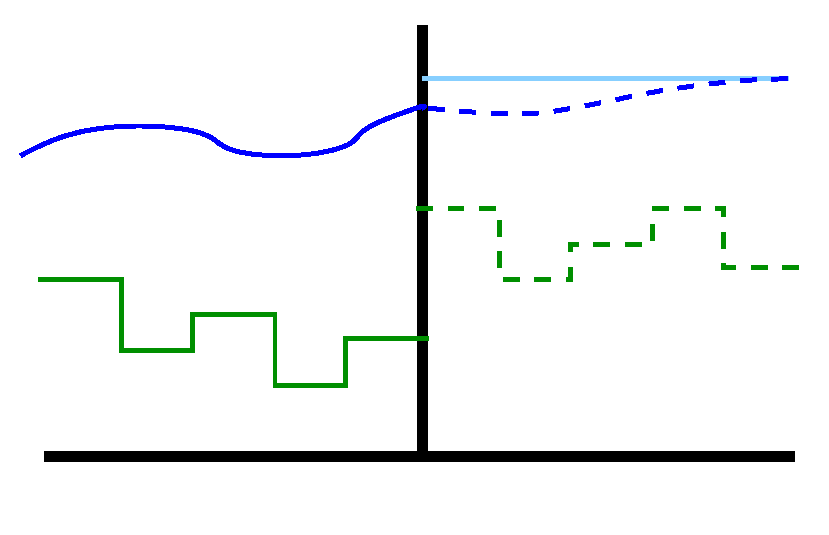
\includegraphics{mpc/MPC_gen}%
\end{picture}%
\setlength{\unitlength}{4144sp}%
%
\begingroup\makeatletter\ifx\SetFigFont\undefined%
\gdef\SetFigFont#1#2#3#4#5{%
  \reset@font\fontsize{#1}{#2pt}%
  \fontfamily{#3}\fontseries{#4}\fontshape{#5}%
  \selectfont}%
\fi\endgroup%
\begin{picture}(6051,3819)(2713,-7190)
\put(2881,-4111){\makebox(0,0)[lb]{\smash{{\SetFigFont{20}{24.0}{\familydefault}{\mddefault}{\updefault}{\color[rgb]{0,0,0}Outputs}%
}}}}
\put(3241,-7081){\makebox(0,0)[lb]{\smash{{\SetFigFont{20}{24.0}{\familydefault}{\mddefault}{\updefault}{\color[rgb]{0,0,0}$\gets$ Past}%
}}}}
\put(2971,-5191){\makebox(0,0)[lb]{\smash{{\SetFigFont{20}{24.0}{\familydefault}{\mddefault}{\updefault}{\color[rgb]{0,0,0}Inputs}%
}}}}
\put(6391,-3751){\makebox(0,0)[lb]{\smash{{\SetFigFont{20}{24.0}{\familydefault}{\mddefault}{\updefault}{\color[rgb]{0,0,0}Setpoint}%
}}}}
\put(6661,-7081){\makebox(0,0)[lb]{\smash{{\SetFigFont{20}{24.0}{\familydefault}{\mddefault}{\updefault}{\color[rgb]{0,0,0}Future $\to$}%
}}}}
\put(5401,-4921){\makebox(0,0)[lb]{\smash{{\SetFigFont{20}{24.0}{\rmdefault}{\mddefault}{\updefault}{\color[rgb]{0,0,0}$u$}%
}}}}
\put(5491,-7081){\makebox(0,0)[lb]{\smash{{\SetFigFont{20}{24.0}{\familydefault}{\mddefault}{\updefault}{\color[rgb]{0,0,0}$k=0$}%
}}}}
\put(5941,-4381){\makebox(0,0)[lb]{\smash{{\SetFigFont{20}{24.0}{\rmdefault}{\mddefault}{\updefault}{\color[rgb]{0,0,0}$y$}%
}}}}
\end{picture}%
}}
\caption{Rolling horizon optimization.}
\label{fig:mpc:mpc_gen}
\end{figure}

Model predictive control technology has two important aspects that are
interconnected. First, is the design of the online optimization
problem that is solved. The design must account for the control
objectives, process constraints and dynamics. Second, is the study of the injected
control moves in the plant. Since only the first input of the optimal
input sequence is used, it is important to provide guarantees that the
control objectives are met in the closed-loop. Stability theory
provides controller design guidelines and theoretical support to
ensure desirable closed-loop behavior by using the rolling horizon
optimization framework.

This chapter is organized as follows. In Section
\ref{sec:mpc:centralized}, we provide an overview of centralized 
MPC. We discuss optimal MPC in Section
\ref{sec:mpc:centralized:optimal} and suboptimal MPC in Section
\ref{sec:mpc:centralized:suboptimal}. In Section
\ref{sec:mpc:distributed}, we introduced distributed MPC; with
noncooperative MPC discussed in Section
\ref{sec:mpc:distributed:ncoop} and cooperative MPC discussed in
Section \ref{sec:mpc:distributed:coop}. An algorithm for robust
cooperative control is presented in Section \ref{sec:mpc:robust}. In
Section \ref{sec:mpc:related}, we discuss related 
work in the field of cooperative/ distributed MPC.  
Since the focus of this thesis is the
application of control technology for supply chain optimization, we
focus our attention on linear models in this section. In Chapter
\ref{chap:sc}, we show that the supply chain dynamics can be described
by linear models. 

\section{Centralized MPC}
\label{sec:mpc:centralized}
\subsection{Preliminaries}
We consider the linear system 
\begin{equation}
\label{eq:mpc:cent_model}
x^+ = Ax + Bu
\end{equation}
in which $x \in \mathbb{R}^n$, $u \in \mathbb{R}^m$ are the states and
inputs while $x^+$ is the successor state.

The system is constrained by the state constraint $x \in \mathbb{X}
\subseteq \mathbb{R}^n$ and input constraint $u \in \mathbb{U}
\subset \mathbb{R}^m$.

For a given finite horizon $N$, we define the input sequence as $\bu =
\left(u(0),u(1),\ldots,u(N-1)\right) \in \mathbb{U}^N$. The state at
time $j \geq 0$ for a system starting at state $x$ at time $j=0$,
under control $\bu$ is given by $\phi(j;x,\bu)$. If there is no
ambiguity, $\phi(j;x,\bu)$ is also denoted as $x(j)$. 

We define the tracking stage cost as $\ell(x,u) = 1/2(x'Qx + u'Ru); Q,R>0 $.  We define an economic state cost $\ell_E(x,u)$ in
Chapter \ref{chap:esc}. Without loss of generality, we assume
that the MPC is designed to track $(x,u)$ to the origin. For systems
in which the 
steady state  is not the origin, we can modify $\ell(x,u)$ by a
simple variable transformation $x \leftarrow x-x_s$, in which $x_s$ is
the steady state  of choice. We also define a terminal cost on the
state, $V_f(x) = 1/2x'Px, P>0$. An important feature of the MPC online optimization problem is the
terminal constraint \eqref{eq:mpc:Xfconst}. The set $\mathbb{X}_f
\subseteq \mathbb{X}$ is the terminal set.

The MPC online optimization problem is now defined as:
\begin{xalignat}{2}
\mathbb{P}_N(x):& \min_{\bu}V_N(x,\bu) & \nonumber \\
&\text{s.t.~} x(j+1) = Ax(j) + Bu(j), &  j =
\set{0,1,2,\ldots,N-1} \nonumber \\
&x(j) \in \mathbb{X} &  j  = \set{0,1,2,\ldots,N} \nonumber\\
&u(j) \in \mathbb{U} &  j =
\set{0,1,2,\ldots,N-1} \label{eq:mpc:PNx} \\
&x(0) = x & \nonumber\\
&x(N) \in \mathbb{X}_f \label{eq:mpc:Xfconst}
\end{xalignat}

In the optimization problem $\mathbb{P}_N(x)$, the cost function
$V_N(x,\bu)$ is given by:
\begin{equation}
\label{eq:mpc:VN}
V_N(x,\bu) = \sum_{j=0}^{N-1} \ell(x(j),u(j)) + V_f(x(N))
\end{equation}




The set $\mathbb{Z}_N$ is defined as the set of $(x,\bu)$ for which the
problem $\mathbb{P}_N(x)$ is feasible. That is,
\begin{equation}
\label{eq:mpc:Z}
\mathbb{Z}_N := \set{(x,\bu) \mid \phi(j;x,\bu) \in \mathbb{X},
  \phi(N;x,\bu) \in \mathbb{X}_f, \bu \in \mathbb{U}^N}
\end{equation}

The projection of set $\mathbb{Z}_N$ onto $\mathbb{X}$ is the set of
admissible states, denoted by $\mathcal{X}_N$. That is, 
\begin{equation}
\label{eq:mpc:X_N}
\mathcal{X}_N := \set{ x \mid \exists \bu \in \mathbb{U}^N,
  \text{~s.t~} (x,\bu) \in \mathbb{Z}_N}
\end{equation}

For a given $x \in \mathcal{X}_N$, the set of feasible inputs is
given by $\mathcal{U}_N(x)$:
\begin{equation}
\label{eq:mpc:U_Nx}
\mathcal{U}_N(x) := \set{ \bu \mid (x,\bu) \in \mathbb{Z}_N}
\end{equation}

The online optimization problem can now succinctly be expressed as:
\[ \mathbb{P}_N(x) := \min_{\bu}{V_N(x,\bu)} \qquad \text{s.t.~} \bu
\in \mathcal{U}_N(x) \]

\subsection{Optimal MPC}
\label{sec:mpc:centralized:optimal}
The following assumptions are made on the system:
\begin{assumption}
\label{ass:mpc:stab}
The centralized system $(A,B)$
is stabilizable.  
\end{assumption}

\begin{assumption}
\label{ass:mpc:psd}
The cost functions $\ell(x,u)$ and $V_f(x)$ are positive definite
\footnote{ A function $f(x)$ is positive definite if $f(x) \geq 0
  \forall x$ and $f(x) = 0$ if and only if $x = 0$.}
\end{assumption}
\begin{assumption}
\label{ass:mpc:bsa}
The set $\mathbb{X}_f$ and the  costs $\ell(x,u), V_f(x)$ are chosen
such that there exists a terminal controller $u = \kappa_f(x)$
that satisfies: 
\begin{xalignat}{1}
\label{eq:mpc:bsa}
V_f(Ax+B\kappa_f(x)) -V_f(x) \leq -\ell(x,\kappa_f(x)) &\qquad \forall x
\in \mathbb{X}_f \\
Ax + B\kappa_f(x) \in \mathbb{X}_f,  \kappa_f(x) \in \mathbb{U}& \qquad
\forall x \in \mathbb{X}_f
\end{xalignat}
\end{assumption} 

\begin{assumption}
\label{ass:mpc:closed}
The set $\mathbb{U}$ is convex, closed and compact and contains the origin in
its interior. The set $\mathbb{X}$ is convex, closed and contains the origin
in its interior. The set $\mathbb{X}_f$ is  convex, closed, compact and
contains the origin in its interior.
\end{assumption}

\begin{remark}
The choice of quadratic stage and terminal costs with $Q > 0, R >0,
P>0$ automatically satisfies Assumption \ref{ass:mpc:psd}.
\end{remark} 

\begin{remark}
From Assumption \ref{ass:mpc:stab}, we know that there exists a linear
feedback $K$ such that $(A+BK)$ is stable. In other words, the
closed-loop $x^+ = (A+BK)x$ is stable. We choose such a $K$ as the
terminal controller $\kappa_f(x)$. The terminal penalty $V_f(x) =
x'Px$ is chosen as 
the solution to the Lyapunov equation (which exists as a consequence
of Assumption \ref{ass:mpc:psd}):
\[ (A+BK)'P(A+BK) + (Q+K'RK) = P \]

For the pair $(P,K)$, we can define the control invariant region in
the state-space in which $u=Kx$ does not activate any constraints as:
\[ \mathbb{X}_f := \set{x \mid x(i) = (A+BK)^ix \in \mathbb{X}_f \subseteq
  \mathbb{X}, Kx(i) \in \mathbb{U}, \forall i \geq 0}
\]

For linear systems, such sets can be easily constructed. See
\citet{gilbert:tan:1991} for an algorithm. 
\end{remark}

The optimal solution to the optimization problem  \eqref{eq:mpc:PNx}
is denoted by 
$\bu^0(x)$ and the optimal objective value is given by $V_N^0(x)$. The
optimal-MPC control law is now defined as $\kappa_o(x) = u^0(0;x)$ in
which $u^0(0;x)$ is the first input in the optimal sequence
$\bu^0(x)$. The closed-loop evolution, under the control law
$\kappa_0(x)$ is $x^+ = Ax + B\kappa_0(x)$. The centralized optimal
MPC asymptotic (exponential) stability theorem is presented below. This theorem is
attributed to \citet[Thm 2.24(b), Chap. 2]{rawlings:mayne:2009}.

\begin{theorem}[Optimal MPC stabilty]
\label{thm:mpc:optimal}
Let Assumptions \ref{ass:mpc:stab}--\ref{ass:mpc:closed} hold. Then
the origin is exponentially stable with a region of attraction
$\mathcal{X}_N$ for the system $x^+ = Ax + B\kappa_0(x)$. If
$\mathcal{X}_N$ is unbounded, then the region of attraction is any
sublevel set of $V_N^0(\cdot)$.
\end{theorem}

The detailed technical proof for Theorem \ref{thm:mpc:optimal} is
provided in \citet[Chap. 2]{rawlings:mayne:2009}. We provide a sketch
of the proof below for linear systems with positive definite stage
cost. The stability proof follows by establishing that 
$V_N^0(\cdot)$ is a 
Lyapunov function for the closed-loop dynamics $x^+=Ax +
B\kappa_0(x)$. 

Lyapunov stability theorem for a dynamic system
$z^+=f(z)$ states that if a function $V(z)$ exists with the following
properties
\begin{gather}
V(z) \geq \alpha_1(\norm{z}), \qquad \forall z \in \mathcal{Z} \label{eq:mpc:lyap:lower-bound} \\
V(z) \leq \alpha_2(\norm{z}), \qquad \forall z \in \mathcal{Z} \label{eq:mpc:lyap:upper-bound}\\
V(z^+) -V(z) \leq -\alpha_3(\norm{z}) \qquad \forall z \in \mathcal{Z} \label{eq:mpc:lyap:cost-drop}
\end{gather}
in which $\alpha_i(\cdot), i \in \set{1,2,3}$ are
$\mathcal{K}_{\infty}$ functions\footnote{A function $\sigma: \mathbb{R}_+
  \rightarrow \mathbb{R}_+$ belongs to the class of
  $\mathcal{K}_{\infty}$ functions if $\sigma$ is continuous, strictly
increasing, $\sigma(0) = 0$ and $\sigma(s) \rightarrow \infty$ as $s
\rightarrow \infty$.}; then the origin is asymptotically
stable on the set $\mathcal{Z}$. Converse Lyapunov theorem states that if the dynamic system is
asymptotically stable, then there exists a Lyapunov function for that
system. If the $\mathcal{K}_{\infty}$ functions $\alpha_i$  are of the
form $\lambda_i \norm{x}^\sigma, \lambda_i,\sigma >0$, then the dynamic
system is exponentially stable (see \citet[Appendix B.]{rawlings:mayne:2009} for precise
statements).

To show that $V_N^0(\cdot)$ is a Lyapunov function for the linear
system under study \footnote{refer to \citet[Chap
  2.]{rawlings:mayne:2009} for more general cases}, we first define
the warm start as follows:
\begin{definition}[Warm Start]
\label{def:mpc:warmstart}
Let $(x,\bu)$ be a state-input vector pair such that $(x,\bu) \in
\mathbb{Z}_N$. Then the warm start for the successor initial state
$x^+ = Ax+B\bu(0;x)$ is defined as:
\begin{equation*}
%\label{eq:warmstart}
\tilde{\bu} = \left (\bu(1;x),\bu(2;x),\ldots,\bu(N;x),u_+\right)
\end{equation*}
in which  $u_+ = \kappa_f(\phi(N;x,\bu))$.
\end{definition}

The lower bound  \eqref{eq:mpc:lyap:lower-bound} for the optimal
function is established by using the 
fact that we choose $Q,R,P>0$ (Assumption \ref{ass:mpc:psd}). By this choice of $Q,R,P$, $V_N(x,\bu)$
is positive definite, and hence $V_N^0(x) \geq
\ell(x,\kappa_0(x))$. Since $\ell(x,u) = 1/2(x'Qx+u'Ru)$, we have that
$\ell(x,u) \geq 1/2x'Qx \geq 1/2\underline{\lambda}_Q\norm{x}^2$. The last
inequality follows from the positive definiteness of $Q$ with
$\underline{\lambda}_Q >0$ denoting the smallest eigen-value of
$Q$. We denote the smallest and largets eigen-value of a matrix
$\mathcal{H}$ by $\underline{\lambda}_\mathcal{H}$ and
$\overline{\lambda}_{\mathcal{H}}$ respectively.

Following the definition of the warm start and an optimal input
sequence $\bu^0(x)$, the warm start $\tilde{\bu}^0$ is feasible for
the successor state $x^+ = Ax+B\kappa_o(x)$, because $x(N) = \phi(N;x,\bu^0)$
belongs to $\mathbb{X}_f$ (and hence $Ax(N)+B\kappa_f(x(N)) \in
\mathbb{X}_f$ by Assumption \ref{ass:mpc:bsa}). Therefore, we get the
following inequality that establishes the cost-drop property in
Equation \eqref{eq:mpc:lyap:cost-drop}.
\begin{gather*}
V_N(x^+,\tilde{\bu}^0) =
V_N^0(x)+\underbrace{\left(V_f(Ax(N)+B\kappa_f(x(N)))
+\ell(x(N),\kappa_f(x(N)))-V_f(x(N))\right)}_{\leq
  0 \text{~by Assumption \ref{ass:mpc:bsa}}} -
\underbrace{\ell(x,\kappa_0(x))}_{\geq 0 \text{~by Assumption
    \ref{ass:mpc:psd}}} \\
V_N^0(x^+) \leq V_N(x^+,\tilde{\bu}^0)\leq  V_N^0(x)
 - \underline{\lambda}_{Q}\norm{x}^2
\end{gather*}

The upper bound \eqref{eq:mpc:lyap:upper-bound} is established by
showing that $V_N^0(x) \leq V_f(x) 
\leq \overline{\lambda}_P\norm{x}^2,
\forall x \in \mathbb{X}_f$. To do so, consider $x \in \mathbb{X}_f$
and choose $u(0) = \kappa_f(x)$. Therefore, $x(1) = Ax+Bu(0)$
satisfies $V_f(x(1))+\ell(x,u(0)) \leq V_f(x)$. Since Assumption
\ref{ass:mpc:bsa} is satisfied, we can choose $u(1) =
\kappa_f(x(1))$ to obtain $x(2) = Ax(1) + Bu(1)$. Therefore
$V_f(x(2))+\ell(x(1),u(1)) \leq V_f(x(1))$. So, we can conclude that
$V_f(x(2))+\ell(x(1),u(1))+\ell(x,u(0)) \leq V_f(x(1))+\ell(x,u(0))
\leq V_f(x)$, using the first inequality. In such a manner, we can
construct an input sequence $\bu_{\kappa_f}(x) := \set{u(j) =
  \kappa_f(x(j))}$, so 
that $V_N(x,\bu_{\kappa_f}) \leq V_f(x)$. Since $\bu_{\kappa_f}$ is a
feasible input sequence, the optimal cost function $V_N(x,\bu^0) \leq
V_N(x,\bu_{\kappa_f}) \leq V_f(x), \forall x \in \mathbb{X}_f$
\citep{pannocchia:rawlings:wright:2011}.  
The upper bound is extended to $\mathcal{X}_N$ using the
compactness of $\mathbb{X}_f$ \citep[Proposition 2.18]{rawlings:mayne:2009}. 

\subsection{Suboptimal MPC}
\label{sec:mpc:centralized:suboptimal}
The favorable properties of the closed-loop was established in optimal
MPC based on the optimal value function. However, in many practical
applications, we might not be able to solve the optimization problem
\eqref{eq:mpc:PNx} to optimality. We might not be able to solve to
optimality in the given sample time (for large 
problems and small sampling time) or by design (like for
example, in cooperative MPC, as we show in Section
\ref{sec:mpc:distributed:coop}). Hence, it is important that asymptotic
stability be ensured when the online optimizations do not converge to
the optimal solution. Suboptimal MPC theory is used to establish this
property. 

Given any feasible input sequence $\bu \in \mathcal{U}_N(x)$ for the
state $x$, the warm start is defined according to Definition
\ref{def:mpc:warmstart}, and the successor input set for the state
$x^+=Ax+Bu(0;x)$ is defined as
below:
\begin{definition}[Successor input set]
\label{def:mpc:successor-input-set}
Consider $(x,\bu)$ such that $\bu$ is feasible for
$\mathbb{P}_N(x)$ \eqref{eq:mpc:PNx}.  For the  successor state 
$x^+ = Ax+Bu(0;x)$, we define the set $G(x,\bu)$
\begin{equation}
\label{eq:mpc:succesor-input-set}
G(x,\bu) = \lbrace \bu^+ \mid \bu^+ \in
\mathcal{U}_N(x^+), V_N(x^+,\bu^+)\leq V_N(x,\tilde{\bu}), 
V_N(x^+,\bu^+) \leq V_f(x^+) \text{~if~} x\in \mathcal{B}_r \subset \mathbb{X}_f \rbrace
\end{equation}
in which $\tilde{\bu}$ is the warm start given by Definition 
\ref{def:mpc:warmstart} and $\mathcal{B}_r$ is a ball of radius $r>0$. We
choose $r$ sufficiently small such that  
$\mathcal{B}_r$ is a subset of the terminal region.  
\end{definition}

Similar to optimal MPC, we inject the first input from the suboptimal
sequence to the plant. The control law in the case of suboptimal MPC
is therefore a set, as any input sequence in the successor input set
can be used. The closed-loop analysis, consequently is on the
evolution of the following system
\begin{align}
x^+ &= Ax+ B\kappa_s(x) \label{eq:mpc:suboptimal:xcl} \\
\bu^+ &\in G(x,\bu)  \label{eq:mpc:suboptimal:ucl}
\end{align}
in which $\kappa_s(x)$ is the control law given by the first input in
the input sequence $\bu(x)$. The following theorem, attributed to
\citet{pannocchia:rawlings:wright:2011} establishes the exponential
stability of suboptimal MPC. Additionally, we make the 
following assumptions on the cost function $V_N(x,\bu)$.

\begin{assumption}
\label{ass:mpc:suboptimalconstants}
There exist positive constants $a,a_1',a_2',a_f$ and $r$, such
that the cost function $V_N(x,\bu)$ satisfies:
\begin{alignat*}{2}
\ell(x,u) &\geq a_1' \norm{(x,u)}^a &\qquad (x,u) &\in \mathbb{X} \times \mathbb{U} \\
V_N(x,\bu) &\leq a_2' \norm{(x,\bu)}^a &\qquad (x,u) &\in
\mathcal{B}_{r} \\
V_f(x) &\leq a_f\norm{x}^a &\qquad x &\in \mathbb{X}
\end{alignat*}
in which $\mathcal{B}_{r}$ is the ball of radius $r$.
\end{assumption}

Note that it is easy to show that Assumption
\ref{ass:mpc:suboptimalconstants} is satisfied for linear systems and
quadratic costs.

\begin{theorem}
\label{thm:mpc:suboptimal}
Let Assumptions \ref{ass:mpc:stab} -- \ref{ass:mpc:closed} and
\ref{ass:mpc:suboptimalconstants} 
hold. For any $x$ for which  $\mathcal{U}_N(x)$  is not empty, choose
$\bu \in \mathcal{U}_N(x)$. Then, the origin of the closed-loop system 
\eqref{eq:mpc:suboptimal:xcl}--\eqref{eq:mpc:suboptimal:ucl}
is asymptotically stable on (arbitrarily large) compact  subsets of
the feasible region $\mathcal{X}_N$
\end{theorem}

We now provide a sketch of the proof for Theorem
\ref{thm:mpc:suboptimal} for linear systems with quadratic,
positive-definite stage costs. We refer the reader to
\citet{pannocchia:rawlings:wright:2011} for  the detailed proof
of a more general case. 
Since in suboptimal MPC, there are multiple input sequences that satisfy
\eqref{eq:mpc:succesor-input-set}, the closed-loop dynamics follows a
difference inclusion, instead of a difference equation. Using the
notation $z = (x,\bu)$ (called as the extended state), the closed-loop
\eqref{eq:mpc:suboptimal:xcl}--\eqref{eq:mpc:suboptimal:ucl} can be
succinctly written as:
\[ z^+ \in H(z) := \set{(x^+,\bu^+) \mid x^+\in Ax+B\kappa_s(x), \bu^+ \in
  G(z)} \]

Analogous to the Lyapunov function described in the previous section;
we can write a Lyapunov function for the difference inclusion. $V(z)$
is an exponential Lyapunov function for $z^+\in H(z)$ on the set
$\mathcal{Z}$ if the following hold, with $a_1,a_2,a_3,a \geq 0$ \citep[Definition
13]{pannocchia:rawlings:wright:2011}. 
\begin{xalignat}{1}
V(z) \geq a_1\norm{z}^a,& \qquad \forall z \in
\mathcal{Z} \label{eq:mpc:Dlyap:lower-bound} \\ 
V(z) \leq a_2\norm{z}^a, &\qquad \forall z \in
\mathcal{Z} \label{eq:mpc:Dlyap:upper-bound}\\ 
\max_{z^+ \in H(z)}{V(z^+)} -V(z) \leq -a_3\norm{z}^a,&  \qquad \forall z \in
\mathcal{Z} \label{eq:mpc:Dlyap:cost-drop} 
\end{xalignat}

Exponential stability is established by showing that $V_N(x,\bu)$ is a
Lyapunov function for the difference inclusion $z^+ \in H(z)$. 
To show that the cost function $V_N(x,\bu)$ satisfies
\eqref{eq:mpc:Dlyap:lower-bound}--\eqref{eq:mpc:Dlyap:upper-bound}, we
proceed by noting that the cost function can be written as:
\begin{equation}
V_N(x,\bu) = \frac{1}{2} \begin{bmatrix} x\\\bu \end{bmatrix}'
\mathcal{H} \begin{bmatrix} x\\\bu \end{bmatrix}  
\qquad 
\mathcal{H} = \begin{bmatrix} \mathcal{A}'\mathcal{Q}\mathcal{A}
  &\mathcal{A}'\mathcal{Q}\mathcal{B}\\
  \mathcal{B}'\mathcal{Q}\mathcal{A} &
  \mathcal{B}\mathcal{Q}\mathcal{B} + \mathcal{R} \end{bmatrix} 
\label{eq:mpc:VN_H}
\end{equation}
in which 
\begin{equation*}
\begin{bmatrix}x(0)\\x(1)\\\vdots\\x(N)\end{bmatrix} =
\underbrace{\begin{bmatrix}I\\A\\\vdots\\A^{N-1}\end{bmatrix}}_{\mathcal{A}}x
+\underbrace{\begin{bmatrix}0&0&\ldots&0\\
B&0&\ldots&0\\AB&B&\ldots&0\\
\vdots&\vdots&\ddots&\ldots\\
A^{N-1}B&A^{N-2}B&\ldots&B\end{bmatrix}}_{\mathcal{B}}\bu  
\end{equation*}
and $\mathcal{Q} = \diag(\underbrace{Q,Q,\ldots,Q}_{N-1 
  \text{~times}},P)$ and $\mathcal{R} =
\diag(\underbrace{R,R,\ldots,R}_{N \text{~times}})$. 
Since $Q,R>0$, the matrix $\mathcal{H}$ is a positive definite
matrix. Therefore, $1/2\underline{\lambda}_{\mathcal{H}}\norm{x,\bu}^2
\leq V_N(x,\bu) \leq \overline{\lambda}_{\mathcal{H}}\norm{x,\bu}^2$
Thus,
\eqref{eq:mpc:Dlyap:lower-bound} and \eqref{eq:mpc:Dlyap:upper-bound}
are satisfied. To show the cost-drop property, notice that for $x \in
\mathcal{B}_r \subset \mathbb{X}_f$, we have by the property of
$G(x,\bu)$ that $V_N(x,\bu) \leq V_f(x)$. As shown in the previous
section, $V_f(x) = 1/2x'Px \leq \overline{\lambda}_P\norm{x}^2$. Hence,
we have that 
\begin{equation}
\label{eq:mpc:suboptimal:inputcost0}
\underline{\lambda}_{\mathcal{H}}\norm{\bu}^2 \leq \underline{\lambda}_{\mathcal{H}}\norm{(x,\bu)}^2 \leq V_N(x,\bu)
\leq V_f(x) \leq  \overline{\lambda}_P\norm{x}^2 ,\qquad x \in
\mathcal{B}_r
\end{equation}
From the inequality \eqref{eq:mpc:suboptimal:inputcost0}, we can conclude that 
\begin{equation}
\label{eq:mpc:suboptimal:inputcost1}
\norm{\bu} \leq d
\norm{x}, \quad x \in \mathcal{B}_r
\end{equation}
in which $d =
\sqrt{\frac{\overline{\lambda}_P}{\underline{\lambda}_{\mathcal{H}}}}$. Using
 inequality \eqref{eq:mpc:suboptimal:inputcost1}, we can establish
 that
\begin{equation}
\label{eq:mpc:suboptimal:inputcost2}
\norm{(x,\bu)} \leq
\norm{x}+\norm{\bu} \leq (1+d)\norm{x} \leq (1+d)\norm{(x,u(0))}
\qquad x \in \mathcal{B}_r
\end{equation}
As we saw in the previous section, $V_N(x^+,\tilde{\bu})-V_N(x,\bu) \leq
-\ell(x,u(0))$ (by choice of the warm start). Since, $\bu^+ \in G(x,\bu)$ implies that (i)
$\bu^+$ drives the state $x^+$ into the terminal region in $N$ steps
and, (ii) ensures that the cost of doing so is less than
$V_N(x^+,\tilde{\bu})$; we can conclude that
\[V_N(x^+,\bu^+)-V_N(x,\bu) \leq -\ell(x,u(0))\]
Note that the lower
bound of $\ell(x,u(0))$ is given by
\[1/2\min{(\underline{\lambda}_Q,\underline{\lambda}_R)}\norm{(x,u(0))}^2
\leq  \ell(x,u(0))\]
Denote $1/2\min{(\underline{\lambda}_Q,\underline{\lambda}_R)} =
a_1'$. Using the inequality \eqref{eq:mpc:suboptimal:inputcost2}, we
can then conclude that 
\[ V_N(x^+,\bu^+)-V_N(x,\bu) \leq -\ell(x,u(0)) \leq
-a_1'\norm{(x,u(0))}^2 \leq \frac{-a_1'}{(1+d)^2}\norm{x,\bu}^2 ,\qquad
\forall x \in \mathcal{B}_r\]

The cost-drop property can be extended to the region of attraction
using compactness of $\mathbb{U}$.

The online optimization problem being solved for suboptimal MPC is 
slightly modified from that of optimal MPC. In Equation
\eqref{eq:mpc:suboptimal:PNx}, we present the optimization problem for
suboptimal MPC.

\begin{equation}
\label{eq:mpc:suboptimal:PNx}
\mathbb{P}_N(x) := \min_{\bu}{V_N(x,\bu)} \qquad \text{s.t.~} \bu
\in \mathcal{U}_N(x), \norm{\bu} \leq d \norm{x}, \text{if~} x \in
\mathcal{B}_r
\end{equation}

For future reference, we define the following set:
\begin{equation}
\label{eq:mpc:UN_sub}
\mathcal{U}_N^{s}(x;r) := \set {u \mid u \in \mathcal{U}_N(x),\norm{\bu} \leq d \norm{x}, \text{if~} x \in
\mathcal{B}_r}
\end{equation}

Note that the constraint on $\norm{\bu}$ is not enforced in practical
implementations as $r>0$ can be chosen arbitrarily small. 

The advantage of using suboptimal MPC is that the we do not have to
wait for the online optimizations to 
converge; and we can inject any suboptimal iterate generated by the
optimization algorithm into the plant as long as that iterate belongs
to the set $G(x,\bu)$. Another important feature that stands out from
the suboptimal MPC theory is that just using the warm start at every
time ensures exponential stability. Online optimization improves the
open-loop prediction cost.\footnote{But we cannot say anything about
  the closed-loop cost if we stop at suboptimal iterates.}




\section{Distributed MPC}
\label{sec:mpc:distributed}
In the previous sections, we introduced centralized MPC, in which a
single controller is designed for the system. The centralized
controller uses system-wide information about models, constraints on
the inputs and states, and objective to find a control law that has favorable properties. In many practical
applications, this centralized information is distributed among many
agents. For example, a chemical plant may have multiple MPC
controllers running, each of which is controlling one process in the
facility. In such cases, it is important to study how to coordinate
information spread among multiple controllers to better control the
plant. Distributed MPC is the study of various architectures for
information sharing and retrieval to coordinate multiple controllers
\citep{scattolini:2009}. 

In this Section, we first introduce the models and objectives of each
agent or node in the system in Section
\ref{sec:mpc:distributed:models}. In Section \ref{sec:mpc:distributed:ncoop}, we describe the
so-called noncooperative MPC, in which the nodes share information
regarding their future (predicted) input moves with each other. In Section
\ref{sec:mpc:distributed:coop}, we present the cooperative MPC
algorithm in which the nodes not only share information about their
predicted input moves with each other, but they also share (and use)
model and objective functions. We show that cooperative MPC is an
implementation of suboptimal centralized MPC, and hence it inherits
all the desirable properties of suboptimal (centralized) MPC. 
We   present a simple  two-tank system shown in Figure
\ref{fig:2tankunstable} in Section
\ref{sec:mpc:distributed:example}. We use this example to illustrate
the key properties of distributed
MPC algorithms, namely (i) noncooperative MPC can de-stabilize a
plant, and (ii) with careful design, cooperative MPC can stabilize any
plant that can be stabilized using centralized MPC. We choose the two-tank system
because its model is a system of integrators like the supply chain
model (see Chapter \ref{chap:sc}).
 
\subsection{Models, constraints and objective functions}
\label{sec:mpc:distributed:models}
In distributed MPC, the system is assumed to be composed of several
subsystems (or agents or nodes). We use the index $i$ to denote a
subsystem, and $M$ to denote the total number of subsystems. Each
subsystem $i \in \set{1,2,3,\ldots,M}$ has the following dynamics
and constraints:
\begin{gather}
\label{eq:mpc:distributed:dynamics}
x_i^+ = A_i x_i + B_{ii} u_i + \sum_{l \in \set{1,2,\ldots,M} \atop l \neq i}
B_{il} u_l \\
x_i \in \mathbb{X}_i \qquad u_i \in
\mathbb{U}_i \label{eq:mpc:distributed:constraints} 
\end{gather}
in which $x_i,u_i$ are the states and inputs in subsystem $i$.

The stage cost for a subsystem is given by:
\begin{equation}
\label{eq:mpc:distributed:stage-cost}
\ell_i(x_i,u_i) = 1/2(x_i'Q_ix_i + u_i'R_iu_i)
\end{equation}
with the penalties $Q_i,R_i >0$. 

The centralized (system-wide) model is therefore:
\begin{gather}
\label{eq:mpc:distributed:cent}
\begin{bmatrix}x_1\\x_2\\\vdots\\x_M\end{bmatrix}^+
= \underbrace{\begin{bmatrix}A_1 & & & \\ & A_2 & & \\ & & \ddots& \\
    & & & A_M \end{bmatrix}}_{A}
\underbrace{\begin{bmatrix}x_1\\x_2\\\vdots\\x_M\end{bmatrix}}_{x}+
\underbrace{\begin{bmatrix}B_{11}&B_{12}&\ldots&B_{1M}\\
B_{21}&B_{22}&\ldots&B_{2M}\\ 
\vdots& \vdots& \ddots& \vdots\\
B_{M1}&B_{M2}& \ldots&B_{MM} \end{bmatrix}}_{B}
\underbrace{\begin{bmatrix}u_1\\u_2\\\ldots\\u_M\end{bmatrix}}_{u} \\
\mathbb{X} = \mathbb{X}_1 \times \mathbb{X}_2 \times \ldots \times
\mathbb{X}_M \\
\mathbb{U} = \mathbb{U}_1 \times \mathbb{U}_2 \times \ldots \times
\mathbb{U}_M
\end{gather}

The centralized stage-cost is 
\begin{equation}
\label{eq:mpc:distributed:cent-stage-cost}
\ell(x,u) = \sum_{i=1}^{M} \ell_i(x_i,u_i)
\end{equation}

We do not make any special assumptions on the local models
\eqref{eq:mpc:distributed:dynamics}--\eqref{eq:mpc:distributed:constraints}. The
only assumptions made are on the centralized model and stage costs
\eqref{eq:mpc:distributed:cent}--\eqref{eq:mpc:distributed:cent-stage-cost}. We
assume that the centralized model and stage costs satisfies Assumptions
\ref{ass:mpc:stab}--\ref{ass:mpc:closed} and \ref{ass:mpc:suboptimalconstants}. It is important to note that
the terminal controller $\kappa_f(\cdot)$, terminal cost $V_f(\cdot)$
and, terminal set $\mathbb{X}_f$ are all defined only for the
centralized system. 


\subsection{Noncooperative MPC}
\label{sec:mpc:distributed:ncoop}
In noncooperative MPC, each subsystem minimizes
its local objective function. Therefore, the subsystem optimization
problem $\mathbb{P}_N^i(x_i,\mathbf{v}_{-i})$ is given below. For subsystem $i$, we use
$-i$ to denote all the other subsystems, i.e.. $-i =
\set{1,2,\ldots,i-1,i+1,\ldots,M}$. 
\begin{xalignat}{2}
\mathbb{P}_{N,nc}^i(x_i;\mathbf{v}_{-i}):& \min_{\bu_i}{\sum_{j=0}^{N-1}
\ell_i(x_i(j),u_i(j)) + V_{f,i}(x_i(N))}& \nonumber\\
&\text{s.t.~} x_{i}(j+1) = A_{ii}x_i(j) + B_{ii}u_i(j) +  \sum_{l \in \set{1,2,\ldots,M} \atop l \neq i}
B_{il} v_l(j) & j = \set{0,1,\ldots,N-1} \nonumber\\
& x_i(j) \in \mathbb{X}_i & j = \set{0,1,\ldots,N-1}  \label{eq:mpc:distributed:ncoop:PNi}\\
& u_i(j) \in \mathbb{U}_i & j = \set{0,1,\ldots,N-1} \nonumber \\
&x_i(0) = x_i \nonumber
\end{xalignat}

We wish to bring the readers attention to two important features of
the ``local'' optimization problem $P_{N,nc}^i(x_i;\mathbf{v}_{-i})$,
 (i) to make accurate predictions of $x_i(j)$, and hence the
cost function, subsystem $i$
needs to know the future (predicted) inputs of all other subsystems,
and (ii) no terminal constraints are enforced \footnote{Although we
  include a terminal penalty, we provide no design methods to find
  a terminal penalty}. 

In noncooperative MPC (Algorithm \ref{alg:mpc:distributed:ncoop}), each
subsystem broadcasts its input sequence prediction. Based on this
prediction, every subsystem solves its local optimization problem. The
final input is a convex combination of the previously broadcast inputs
and the optimized inputs. 

%\begin{algo}[Noncooperative MPC]\mbox{ }
%\label{alg:mpc:distributed:ncoop}

\begin{algorithm}
  \KwData{Starting state $\set{x_i(0)}$, initial guess $\left(\tilde{\bu}_1(0),
    \tilde{\bu}_2(0),\ldots,\tilde{\bu}_M(0)\right)$, $\bar{p} \geq
  0$, $\omega_i \in (0,1)$ such that $\sum_{i=0}^{M}\omega_i = 1$}
  \KwResult{Closed loop $x(j),u(j)$, $j = \set{0,1,2,\ldots}$}
   Set $j \leftarrow 0$ \\
    \While {$j \geq 0$}{
      Set $p \leftarrow 0$\\
      Set $x_i \leftarrow x_i(j))$, for i in $1,2,\ldots,M$\\
      Set $\tilde{\bu}_i \leftarrow \tilde{\bu}_i(j)$, for i in $1,2,\ldots,M$\\
      Broadcast $\tilde{\bu}_i$ to all other subsystems for  i in
      $1,2,\ldots,M$\\
      Each subsystem $i$ creates $\tilde{\bu}_{-i}$ from the other
      subsystem inputs\\
      \While {$p < \bar{p}$}{
       Solve $\mathbb{P}_{N,nc}^{i}(x_i,\bu_{-i})$ to obtain
       $\bu_i^0$ for i in $1,2,\ldots,M$ \\
       Set $\bu_i^{(p+1)} \leftarrow \omega_i \bu_i^{(p)} +
       (1-\omega_i) \bu_i^0$ for  i in $1,2,\ldots,M$ \\
        Set $p \leftarrow p+1$\
   }
   Set input $u_i(j) = \bu_i(0)$ for i in $ 1,2,\ldots,M$ and
   broadcast \\
   Evolve state from $x_i(k)$ to $x_i(k+1)$ for the input just
   obtained \\
   Obtain feasible input $\tilde{\bu}_i(j+1)$ for i in $1,2,\ldots,M$\\
   Set $j \leftarrow j+1$
   }
\caption{Noncooperative MPC}
\label{alg:mpc:distributed:ncoop}
\end{algorithm}
%\end{algo}

In the inner loop of Algorithm \ref{alg:mpc:distributed:ncoop}, each
subsystem is finding its {\em{best response}} to the other subsystem
inputs. It can be shown that as $p \rightarrow \infty$, the
solutions $\bu_i^{(p)}$ converge to a point called the Nash
Equilibrium \citep{basar:olsder:1999}. As has been shown earlier by
\citet[Sec 4.3.1]{venkat:2006}, the Nash equilibrium may be
unstable. We also wish to point out that we cannot make any claims
about the feasibility of $\mathbb{P}_N^i(x_i;\mathbf{v}_{-i})$ in the
inner optimization loop of the noncooperative MPC algorithm. For
similar reasons, we cannot make any claims about how to obtain
$\tilde{\bu}_i(j+1)$.

In Figure \ref{fig:mpc:unstable}, we show the unstable closed-loop response using Algorithm
\ref{alg:mpc:distributed:ncoop} for a simple two-tank example.

\subsection{Cooperative MPC}
\label{sec:mpc:distributed:coop}
In this section, we tailor the distributed MPC algorithm to be an
implementation of suboptimal MPC. To do so, we require that the
subsystems not only share input forecasts, but also model, constraints
and objective functions with each other. Under this requirement, the
cooperative MPC optimization problem is written as:

\begin{equation}
\label{eq:mpc:distributed:coopPNx}
\mathbb{P}_N(x) := \min_{\bu}{V_N(x,\bu)} \qquad \text{s.t.~} \bu
\in \mathcal{U}^s_N(x;r)
\end{equation}

Note that the cooperative MPC optimization problem is the same as the
suboptimal MPC optimization problem. The cooperative MPC algorithm is
presented in Algorithm \ref{alg:mpc:distributed:coop}.

%\begin{algo}[Cooperative MPC] \mbox{ }
%\label{alg:mpc:distributed:coop}

\begin{algorithm}
 \KwData{Starting state $x(0)$, initial guess
   $(\tilde{\bu}_1(0),\tilde{\bu}_2(0),\ldots,\tilde{\bu}_M(0)) \in \mathcal{U}^s_N(x(0);r)$,
   $\bar{p} \geq 1$ and $\omega_i \in (0,1)$ such that
   $\sum_{i=0}^{M}\omega_i = 1$}
 \KwResult{Closed loop $(x(j),u(j)), j = \set{1,2,\ldots}$}
 set $j \leftarrow 0$ \\
 \While {$j \geq 0$}{
   Set $p \leftarrow 0$, $x \leftarrow x(j)$\\
   Set $\bu_i^{(p)} \leftarrow \tilde{\bu}_i(j)$ for $i = 1,2,\ldots,M$\\
   Broadcast current subsystem inputs $\tilde{\bu}_i(j)$ to other
   subsystems \\
   \While {$p < \bar{p}$}{
       Solve $\min_{\bu_i}{V_N(x,\bu)} \quad \text{s.t.~} \bu \in
       \mathcal{U}_N^s(x;r); \bu_{-i} = \bu_{-i}^{(p)}$ to obtain
       $\bu_i^0$ for i in $1,2,\ldots,M$ \\
       Set $\bu_i^{(p+1)} \leftarrow \omega_i \bu_i^{(p)} +
       (1-\omega_i) \bu_i^0$ for i in $1,2,\ldots,M$ \\
       Set $p \leftarrow p+1$\\
   }
  Set $\bu \leftarrow (\bu_1^{(p)},\bu_2^{(p)},\ldots,\bu_M^{(p)})$ and find $x(j+N) \leftarrow
  \phi(N;x(j),\bu)$\\
  Obtain $u_+ = (u_{1+},u_{2+},\ldots,u_{M+}) \leftarrow \kappa_f(x(j+N))$\\
  Obtain warm start $\tilde{\bu}_i(j+1) =
    (\bu_i^{(p)}(1),\bu_i^{(p)}(2),\ldots,u_{i+})$ for $i = 1,2,\ldots,M$.\\
   Set input as $u(j) =
  (\bu_1^{(p)}(0),\bu_2^{(p)}(0),\ldots,\bu_M^{(p)}(0))$\\
  Evolve state from $x(j)$ to $x(j+1)$ under input $u(j)$\\
  Set $j \leftarrow j+1$ \\
 }
\caption{Cooperative MPC}
\label{alg:mpc:distributed:coop}
\end{algorithm}
%\end{algo}

In the inner loop in  Algorithm \ref{alg:mpc:distributed:coop}, all the
subsystems are solving the same optimization problem, but by fixing
the decisions of other sthe ubsystems at the values broadcast in the 
previous iterate. The inner loop is an implementation of the
Jacobi parallel optimization routine \citep[Section
3.3.5]{bertsekas:tsitsiklis:1989}. For convex optimization problems,
the Jacobi algorithm has the property that it generates feasible
iterates with non-increasing objective function values. Before
presenting the cooperative MPC stability theorem
(which in different forms have been stated in
\citet{stewart:venkat:rawlings:wright:pannocchia:2010, venkat:2006, stewart:wright:rawlings:2011, subramanian:rawlings:maravelias:2012}), we
briefly review the properties of Jacobi algorithm for convex
optimization problem.

\subsubsection*{Jacobi algorithm}
For the sake of simplicity, we consider only two subsystems in this
section. Consider the following optimization problem
\eqref{eq:mpc:distributed:coop:jordan}, solved using 
Algorithm \ref{alg:mpc:distributed:coop:jordan}.

\begin{equation}
\label{eq:mpc:distributed:coop:jordan}
\mathbb{J} : \min_{y_1,y_2}{J(y_1,y_2)} \qquad \text{s.t.~} (y_1,y_2)\in \Omega 
\end{equation}
in which $J(\cdot)$ is a convex function and $\Omega$ is a convex,
closed and compact set. 

%\begin{algo}[Jacobi algorithm \citep{bertsekas:tsitsiklis:1989}] \mbox{ }
%\label{alg:mpc:distributed:coop:jordan}

\begin{algorithm}[H]
 \KwData{Starting guess $(y_1,y_2) \in \Omega$
    and $\omega_i \in (0,1)$ such that
   $\sum_{i=1}^{2}\omega_i = 1$}
 \KwResult{Sequence of feasible iterates $\set{y^{(p)}}$ and
   non-increasing objective function values $\set{J(y^{(p)})}$}
 Set $p \leftarrow 0$\\
  \While {$p \geq 0$}{
   Set  $y_1^{(p)} \leftarrow y_1$, $y_2^{(p)}
   \leftarrow y_2$\\
   Solve $\min_{y_1}{J(y_1,y_2)}, \text{s.t.~} y_2 = y_2^{(p)},
   (y_1,y_2) \in \Omega$  to obtain $y_1^0$. \\
   Solve $\min_{y_2}{J(y_1,y_2)}, \text{s.t.~} y_1 = y_1^{(p)},
   (y_1,y_2) \in \Omega$  to obtain $y_2^0$. \\
   Set $y_i^{(p+1)} \leftarrow \omega_i y_i^{(p)} +
       (1-\omega_i) y_i^0$  for i in $1,2$ \\
       Set $p \leftarrow p+1$\\
   }
\label{alg:mpc:distributed:coop:jordan}
\caption{Jacobi algorithm}
\end{algorithm}
%\end{algo}

The following Proposition establishes that  the Jacobi algorithm
generates feasible iterates that have non-increasing objective
function values
\begin{proposition}
\label{prop:mpc:distributed:jordan}
Let $J(y)$ be continuously differentiable and strongly
convex\footnote{Strongly convex implies that $J(\lambda w +
  (1-\lambda)v)  < \lambda J(w) + (1-\lambda)J(v), \forall \lambda \in
  (0,1)$} on the convex, closed and  compact set $\Omega$.
Let Algorithm \ref{alg:mpc:distributed:coop:jordan} be used to solve
convex optimization problem \eqref{eq:mpc:distributed:coop:jordan}
from an initial feasible point $y \in \Omega$. Then, (i) every iterate
$y^{(p)}$ generated by the algorithm is feasible and , (ii)
$J(y^{(p+1)}) \leq J(y^{(p)}), \forall p>0$.
\end{proposition}
The proof is provided in  \citet{stewart:venkat:rawlings:wright:pannocchia:2010}.

While Proposition \ref{prop:mpc:distributed:jordan} is enough to
establish stability of suboptimal MPC, we require the following
proposition to establish that the optimizations in cooperative MPC
converge to the optimal solution. Note that the in contrast to
Proposition \ref{prop:mpc:distributed:jordan}, we require a much
stricter condition on the constraints in Proposition
\ref{prop:mpc:distributed:jordan:converge}, namely that, the
constraints be uncoupled. 

\begin{proposition}
\label{prop:mpc:distributed:jordan:converge}
Let $J(y)$ be continuously differentiable and strongly
convex. Let $\Omega = \Omega_1 \times \Omega_2$, in which $y_1 \in
\Omega_1$ and $y_2 \in \Omega_2$, with $\Omega_i$  convex, closed and compact. Then, as $p
\rightarrow \infty$, the iterates $y^{(p)}$ converges to the $y^o$, in
which $y^o$ is the optimal solution to optimization problem
\eqref{eq:mpc:distributed:coop:jordan}
\end{proposition}  
This proof is provided in  \citet{stewart:venkat:rawlings:wright:pannocchia:2010}. Another
proof is also provided in \citet[Prop 3.9]{bertsekas:tsitsiklis:1989}
for Gauss-Seidel algorithm which is closely related to the Jacobi
algorithm. 

We now present the exponential stability of the cooperative MPC algorithm.
\begin{theorem}
Let Assumptions \ref{ass:mpc:stab} -- \ref{ass:mpc:closed} and
\ref{ass:mpc:suboptimalconstants} 
hold. Choose $r>0$ such that $\mathcal{B}_r \subset \mathbb{X}_f$. For
any $x$ for which  $\mathcal{U}_N^s(x;r)$  is not empty, choose 
$\bu \in \mathcal{U}_N^s(x;r)$. Then, the origin of the closed-loop system 
obtained by Algorithm \ref{alg:mpc:distributed:coop}
is exponentially stable. The region of attraction are (arbitrarily large) compact  subsets of
the feasible region \[\mathcal{X}_N :=\set{x\mid \exists u \in
 \mathbf{U}^N, \text{~s.t~} \mathcal{U}^s_N(x;r) \neq \varnothing}\]
\begin{proof}
We show that the closed-loop system obtained by Algorithm
\ref{alg:mpc:distributed:coop} is an implementation of suboptimal MPC
and use Theorem \ref{thm:mpc:suboptimal} to prove exponential stability. 



We note that the optimization problem \eqref{eq:mpc:distributed:coopPNx} 
has convex constraints and a strongly convex objective. By choice
$Q,R,P>0$, we know that the Hessian $\mathcal{H}$
\eqref{eq:mpc:VN_H} is positive definite, and hence strongly
convex. From Assumption \ref{ass:mpc:closed}, the set $\mathbb{Z}_N$ is
convex and hence the set $\mathcal{U}_N(x)$ is convex too. The set
$\mathcal{U}_N^{s}(x;r)$ is the intersection of two convex
sets. Hence, by Proposition \ref{prop:mpc:distributed:jordan}, we know
that  if $(x,\tilde{\bu})$ is feasible for
\eqref{eq:mpc:distributed:coopPNx} then (i) {\emph{all}} the iterates generated by the inner loop in  Algorithm
\ref{alg:mpc:distributed:coop} are feasible; implying $\bu^{(p)} \in
\mathcal{U}_N^{s}(x;r)$ and, (ii) the cost at iterate $p$ is not
greater than the cost achieved by $V_N(x,\tilde{\bu})$; that is
$V_N(x,\bu^{(p)}) \leq V_N(x,\tilde{\bu})$. 

By choice of $\tilde{\bu}(0)$, we know that $(x(0),\tilde{\bu}(0))$ is
feasible for \eqref{eq:mpc:distributed:coopPNx}. Therefore,
$(x(0),\bu^{(p)}(0)) \in \mathbb{Z}_N$ with $V_N(x(0),\bu^{(p)}(0))
\leq V_N(x(0), \tilde{\bu}(0))$. Since $\tilde{\bu}(1)$ is the warm
start constructed from $\bu^{(p)}(0)$, we know that it is feasible and
that $\tilde{\bu}(1) \in G(x(0),\bu^{(p)}(0))$. Therefore, by induction
the closed-loop obtained by
Algorithm \ref{alg:mpc:distributed:coop} belongs to the family of
closed-loop solutions for which we showed exponential stability in
Theorem \ref{thm:mpc:suboptimal}.
\end{proof}
\end{theorem}

The main difference between cooperative and noncooperative MPC is that
in the inner optimization loop of cooperative MPC, all the subsystems
minimize the centralized problem, but subject only to their
inputs. Therefore, we were able to use warm start and properties of
Jacobi algorithm to establish the cost-drop properties required to
prove exponential stability. 

The cooperative MPC algorithm has the following key properties:
\begin{enumerate}
\item The nominal closed-loop  is exponentially stable.
\item The subsystems need to share models and objective functions with
  each other.
\item There is no coordinator. At the end of every cooperative MPC
  iteration, the subsystems just need to transfer information
  regarding their predicted inputs with each other.
\item There is no minimum number of iterations of the inner-loop that
  is required. Subsystems can choose to stop after any number of
  iterations.

\end{enumerate}

While, we used Proposition \ref{prop:mpc:distributed:jordan} to
establish recursive feasibility and cost-drop of cooperative MPC, we
cannot use Proposition \ref{prop:mpc:distributed:jordan:converge} to establish
that the as $p \rightarrow \infty$, the solution obtained by the
cooperative MPC optimizations converge to the centralized MPC
optimization problem because the constraint set $\bu = (\bu_1,\bu_2,\ldots,\bu_M) \in
\mathcal{U}_N^s(x;r)$ is a coupled constraint. The optimization
problem \eqref{eq:mpc:distributed:coopPNx} can be 
written as
\begin{xalignat}{2}
\mathbb{P}_N(x):& 1/2\begin{bmatrix}x\\\bu\end{bmatrix}'\mathcal{H}
\begin{bmatrix}x\\\bu\end{bmatrix}& \nonumber \\
&\text{s.t.~} x(j) \in \mathbb{X} & j \in 0,1,\ldots,N-1 \nonumber \\
& u(j) \in \mathbb{U} & j \in
0,1,\ldots,N-1\nonumber\\
& \begin{bmatrix} A^{N-1}B & A^{N-2}B & \ldots & B\end{bmatrix}\bu \in
\mathbb{X}_f & \label{eq:mpc:distributed:coop_show_couple}\\
& \norm{\bu} \leq d \norm{x} & x \in \mathcal{B}_r \nonumber
\end{xalignat}

In the following sections, we describe methods
to ``decouple'' the constraint set, so that, in addition to 
establishing stability, we can also establish that the inner-loop
optimizations converge to the centralized optimal solution. Hence, we
can establish that centralized optimal and (converged) cooperative control have
the same feedback solution.

In order to do so, we make the following assumptions for cooperative
MPC:
\begin{assumption}
\label{ass:mpc:noX}
There are no state constraints. State constraints are enforced as
soft penalties by tuning the $Q$ matrix in the stage cost.
\end{assumption}

\begin{assumption}
\label{ass:mpc:uncoupledU}
The input constraint space is uncoupled. That is, the input constraint
set $\mathbb{U}$ is the Cartesian product of the input constraint sets
of each subsystem. 
\[ \mathbb{U} = \mathbb{U}_1 \times \mathbb{U}_2 \times \ldots \times
\mathbb{U}_M
\]
The sets $\mathbb{U}_i$ are convex, closed, compact and, contain the origin in its interior.
\end{assumption}

Using Assumption \ref{ass:mpc:noX}, the state constraints in
\eqref{eq:mpc:distributed:coop_show_couple} are removed. Assumption
\ref{ass:mpc:uncoupledU} ensures that the input constraints for
subsystem $i, i = 1,2,\ldots,M$ do not affect any other subsystems'
input constraints. Although, for most practical applications, we do
not require the constraint $\norm{\bu} \leq d\norm{x}$, we can
easily separate the constraint by enforcing $\norm{\bu_i} \leq
d_i\norm{x}$ such that $\sum_i d_i \leq d$.

Stability requirements mean that we cannot remove the stability
constraint $x(N) \in \mathbb{X}_f$ from the optimization problem. 
In the next two sections, we briefly review
two techniques to ``uncouple'' the terminal region constraint. The
advantage of using the cooperative MPC formulations without coupled
terminal constraints is that we have a ``performance guarantee'' that
the open-loop cost attained by the cooperative MPC algorithm at
convergence is equal to the optimal centralized 
open-loop cost.

\subsubsection{Sub-states}
\label{sec:mpc:distributed:substate}
This relaxation was proposed by
\citet{stewart:venkat:rawlings:wright:pannocchia:2010}, to solve the
terminal equality constraint problem, i.e.,  $\mathbb{X}_f =
\set{0}$. The centralized optimization problem is \footnote{To
  simplify the discussion, we
  enforce the constraint that all the states are zero at the end of
  the horizon. In
  \citet{stewart:venkat:rawlings:wright:pannocchia:2010}, only the
  unstable modes were forced to be zero at the end of the horizon}:
\begin{xalignat}{2}
\mathbb{P}_N(x):& \min_{\bu}V_N(x,\bu) & \nonumber \\
&\text{s.t.~} x_i(j+1) = A_ix_i(j) + B_{ii}u_i(j) +
\sum_{l\in\set{1,2,\ldots,M}\atop l\neq i}B_{il}u_l(j), &  j =
\set{0,1,2,\ldots,N-1},i= \set{1,2,\ldots,M} \nonumber \\
&u_i(j) \in \mathbb{U}_i &  j =
\set{0,1,2,\ldots,N-1}, i = \set{1,2,\ldots,M} \nonumber \\
&x_i(0) = x_i & i = \set{1,2,\ldots,M} \nonumber\\
&x_i(N) = 0 & i= \set{1,2,\ldots,M}  \label{eq:mpc:distributed:substate:PNx}
\end{xalignat}

Notice that the only coupled constraint is $x_i(N) = 0$, as the
dynamics $x^+=Ax+Bu$ can be projected out, i.e., we use the
optimization problem formulation \eqref{eq:mpc:distributed:coop_show_couple}.

We consider a non-minimal realization of the system \eqref{eq:mpc:distributed:dynamics}
such that ``sub-state'' $x_{il}$ in subsystem $i$ is only influenced
by input $l$.
\begin{equation}
\tilde{x}^+_{il} = \tilde{A}_{il}\tilde{x}_{il} + \tilde{B}_{il}u_l 
\end{equation}
Defining $\hat{x}_i = \begin{bmatrix} \set{\tilde{x}_{il}}, l =
  {1,2,\ldots,M}\end{bmatrix}$, each subsystem model is given by
  \eqref{eq:mpc:distributed:dynamics}. The matrices
  $\hat{A}_i,\hat{B}_{il}$ are used to describe the dynamics in
  subsystem $i$.
\begin{gather}
\underbrace{\begin{bmatrix} \tilde{x}_{i1}\\\tilde{x}_{i2} \\\vdots\\\tilde{x}_{iM}\end{bmatrix}^+}_{\hat{x}_i^+} =
 \underbrace{\begin{bmatrix} \tilde{A}_{i1} &  & & \\
  & \tilde{A}_{i2}& & \\
  & & \ddots & \\ & & &\tilde{A}_{iM} \end{bmatrix}
 }_{\hat{A}_i}
 \underbrace{\begin{bmatrix} \tilde{x}_{i1}\\
 \tilde{x}_{i2} \\
 \vdots\\
 \tilde{x}_{iM}
 \end{bmatrix}}_{\hat{x}_i}+
 \underbrace{\begin{bmatrix}\tilde{B}_{i1}\\0\\\vdots\\0\end{bmatrix}}_{\hat{B}_{i1}}u_1
 +
 \underbrace{\begin{bmatrix}0\\\tilde{B}_{i2}\\\vdots\\0\end{bmatrix}}_{\hat{B}_{i2}}u_2
 + \ldots
 \underbrace{\begin{bmatrix}0\\0\\\vdots\\\tilde{B}_{iM}\end{bmatrix}}_{\hat{B}_{iM}}u_M
 \label{eq:mpc:distributed:subsystem}
\\
x_i = \underbrace{\begin{bmatrix} \tilde{C}_{i1} & \tilde{C}_{i2} & \ldots & \tilde{C}_{iM}\end{bmatrix}}_{\hat{C}_i}\underbrace{\begin{bmatrix} \tilde{x}_{i1}\\
\tilde{x}_{i2} \\
\vdots\\
\tilde{x}_{iM} \end{bmatrix}}_{\hat{x}_i}
\end{gather}

We assume that the centralized states $x_i$ can be
constructed from the sub-states $\hat{x}_{i}$. In general, we would
require that the outputs measured in subsystem $i$, $y_i$ can be
reconstructed from the sub-states (see Assumption
\ref{ass:mpc:distributed:substate:stab}).

The subsystem stage cost $\ell_i(x_i,u_i) = 1/2(x_i'Q_ix_i + u_iR_iu_i)$
can now be written as 
\[ \ell_i(x_i,u_i) = \ell_i(\hat{x}_i,u_i) = 1/2(\hat{x}_i \hat{C}_i'Q\hat{C}_i \hat{x}_i +
u_iR_iu_i)\]

The centralized stage cost is $\ell(x,u) = \sum_{i=1}^{M}
\ell_i(\hat{x}_i,u_i)$. Since, we use a terminal constraint that all
states are zero at the end of the horizon, we do not need a terminal penalty.
 
We define $\underline{x}_l$ as the sub-states that are affected by
input $l$. That is $\underline{x}_l = \begin{bmatrix}\set{\tilde{x}_{il}} i =
  \set{1,2,\ldots,M}\end{bmatrix}$. Correspondingly, we define
$\underline{A}_l,\underline{B}_l$ as follows:

\begin{equation}
\underbrace{\begin{bmatrix}
\tilde{x}_{1l}\\
\tilde{x}_{2l}\\
\vdots\\
\tilde{x}_{Ml}
\end{bmatrix}^+}_{\underline{x}_l^+} =
\underbrace{\begin{bmatrix}
\tilde{A}_{1l} & & & \\
& \tilde{A}_{2l} & &  \\
& & \ddots & \\
& & & \tilde{A}_{Ml}
\end{bmatrix}
}_{\underline{A}_l}
\underbrace{\begin{bmatrix}
\tilde{x}_{1l}\\
\tilde{x}_{2l}\\
\vdots\\
\tilde{x}_{Ml}
\end{bmatrix}}_{\underline{x}}
+\underbrace{\begin{bmatrix}
\tilde{B}_{1l}\\
\tilde{B}_{2l}\\
\vdots\\
\tilde{B}_{Ml}
\end{bmatrix}
}_{\underline{B}_l}u_l
\label{eq:mpc:distributed:substate:Aunderline}
\end{equation}


The constraint $x_i(N)=0$ can be equivalently written as $\tilde{x}_{il}= 0, l
\in \set{1,2,\ldots,M}$. Therefore, the centralized MPC problem can be written as:

\begin{xalignat}{2}
\mathbb{P}_N(x): & \min_{\bu}V_N(x,\bu)& \nonumber \\
&\text{s.t.~} \underline{x}_l(j+1) = \underline{A}x_l(j) +
\underline{B}_l(j) u_l(j) &j = \set{0,1,2,\ldots,N-1},l =
\set{1,2,\ldots,M} \nonumber \\
&x_i(j) = \hat{C}_i \hat{x}_i(j) &j = \set{1,2,\ldots,N}, i =
\set{1,2,\ldots,M} \nonumber\\
&u_l(j) \in \mathbb{U} &  j =
\set{0,1,2,\ldots,N-1}, l = \set{1,2,\ldots,M} \nonumber \\
&x_i(0) = x_i & i = \set{1,2,\ldots,M} \nonumber \\
&\underline{x}_l(N) = 0 & l= \set{1,2,\ldots,M}  \label{eq:mpc:distributed:substate:PNx:uncoupled}
\end{xalignat}

In the optimization problem the terminal condition is uncoupled
because the dynamics of state $\underline{x}_l$ depends only on input
$u_l$ via equation \eqref{eq:mpc:distributed:substate:Aunderline}. 
 If Assumption \ref{ass:mpc:distributed:substate:stab} is
satisfied, then  Algorithm \ref{alg:mpc:distributed:coop} can be used to
stabilize the plant {\em{with guaranteed performance}} to the
centralized solution of the problem \eqref{eq:mpc:distributed:substate:PNx} as
there are no coupled constraints in the problem.

Assumption \ref{ass:mpc:distributed:substate:stab} ensures that (i) the input $\bu_i$ can be used to
zero all the states that $u_i$ influences, (ii) all the substates can be
reconstructed from the outputs.

\begin{assumption}[Subsystem stabilizability]\mbox{ }
\label{ass:mpc:distributed:substate:stab}
\begin{itemize}
\item The system $(\underline{A}_i,\underline{B}_i)$ is stabilizable.
\item The system $(\hat{A}_i,\hat{C}_i)$ is detectable.
\end{itemize}
\end{assumption}

We now discuss the features of the aforementioned decomposition:

\paragraph{Applicability.} The decomposition into the substate models
\eqref{eq:mpc:distributed:dynamics} can be obtained from the Kalman decomposition of
the original input/output $y_i,u_i$ model
\citep[p.270]{antsaklis:michel:1997}.

The drawback however, is that not all centralized stabilizable models
have a corresponding substate non-minimal realization that satisfies
Assumption \ref{ass:mpc:distributed:substate:stab}. One such example is the system of
integrators (like supply chain models).

\paragraph{Convergence.} The decomposition ensures that if the inner
optimization loop in Algorithm \ref{alg:mpc:distributed:coop} is allowed to converge,
then the solution is the centralized solution to the optimization
problem \eqref{eq:mpc:distributed:substate:PNx}.

\paragraph{Initialization.} The optimization loop in Algorithm
\ref{alg:mpc:distributed:coop} requires a feasible starting point. The feasible
starting point is ensured by the warm start. The warm start
is feasible because we assume that the actual plant state at the next
sampling time is equal to the model prediction for the next state. In
many applications, when there are plant-model mismatches or unmodeled
disturbances affecting the system, the assumption that the plant
state is equal to the predicted state  breaks down. In such cases,
the warm start can become infeasible and we need a distributed
initialization routine to recover feasibility.

In the substate decomposition of the model, the warm start is
infeasible if $\tilde{x}_{il}(N;x,\bu) \neq 0$ for some
$i,l$. However, since $\tilde{x}_{il}(N;x,\bu)$  depends only on the
input sequence from a single subsystem $\bu_l$, the re-initialization
routine is also decoupled. 

\subsubsection{Relaxing the terminal region}
\label{sec:mpc:distributed:relaxation}
This relaxation was proposed by
\citet{rawlings:stewart:wright:mayne:2010}, and has been used for
nonlinear suboptimal/ distributed / economic  MPC in
\citet{stewart:wright:rawlings:2011},
\citet{pannocchia:rawlings:wright:2011},
\citet{amrit:rawlings:angeli:2011} as well as linear MPC in
\citet{subramanian:rawlings:maravelias:2012}.

In this section, we work with the  centralized model
\eqref{eq:mpc:distributed:dynamics}. The idea here is to develop an optimization problem
without terminal constraints such that every  iterate generated
in the inner optimization loop of Algorithm \ref{alg:mpc:distributed:coop} lies inside
a terminal region that satisfies Assumption \ref{ass:mpc:bsa}. To do so,
we modify (i) the terminal region (ii) the cost function and (iii) the
feasible set as follows:

The terminal region is chosen as a sublevel set of the terminal
cost. That is,

\begin{equation}
\label{eq:mpc:distributed:relaxation:Xfa}
\mathbb{X}_f := \set{x \mid V_f(x) \leq a, a > 0}
\end{equation}

For linear systems, we could use $P$, the solution to the Lyapunov
equation as $V_f(x)$ and choose $a$ such that all the requirements in
Assumption \ref{ass:mpc:bsa} are satisfied.

The cost function is modified so that the terminal penalty is
magnified. That is,

\begin{equation}
\label{eq:mpc:distributed:relaxation:VNbeta}
V^\beta_N(x,\bu) = \sum_{j=0}^{N-1} \ell(x(i),u(i)) + \beta V_f(x(N))
\end{equation}
in which $\beta \geq 1$.

Finally, the feasible set is modified as follows:
\begin{equation}
\label{eq:mpc:distributed:relaxation:ZNbeta}
\mathbb{Z}_N^\beta= \set{ (x,\bu) \mid V_N^\beta(x,\bu) \leq \bar{V}, \bu \in
  \mathbb{U}^N}
\end{equation}
in which $\bar{V} \geq 0$  can be chosen arbitrarily large.

In Proposition \ref{prop:mpc:distributed:relaxation:betabar}, we show how the parameter $\beta$
can be chosen so that if $(x,\bu) \in \mathbb{Z}_N^\beta$, then
$x(N;x,\bu) \in \mathbb{X}_f$. Using  Proposition
\ref{prop:mpc:distributed:relaxation:cost-drop} \footnote{see also
  \citet[Exercise 2.11, Page 177]{rawlings:mayne:2009}}, we can establish that the
warm start given by Definition \ref{def:mpc:warmstart} satisfies the
cost-drop property, i.e., $V_N^\beta(x,\tilde{\bu}) \leq
V_N^\beta(x,\bu)$. 

\begin{proposition}
\label{prop:mpc:distributed:relaxation:betabar}
Let Assumption \ref{ass:mpc:psd} hold. Define the terminal region $\mathbb{X}_f$
according to \eqref{eq:mpc:distributed:relaxation:Xfa}
Let the cost function  $V_N^\beta(x,\bu)$ be given by 
\eqref{eq:mpc:distributed:relaxation:VNbeta}. For  $\bar{V} 
\geq a $, define $\bar{\beta} := \bar{V}/a$. Then, for any $\beta \geq
\bar{\beta}$ and $(x,\bu) \in \mathbb{Z}_N^\beta$ \eqref{eq:mpc:distributed:relaxation:ZNbeta}, we have
that $\phi(N;x,\bu) \in \mathbb{X}_f$.
\begin{proof}
For sake of contradiction, assume that $(x,\bu) \in
\mathbb{Z}_N^\beta$, $\beta \geq \bar{\beta}$, but $\phi(N;x,\bu)
\notin \mathbb{X}_f$, that is $V_f\left(\phi(N;x,\bu)\right)>a$. Since
$(x,\bu) \in \mathbb{Z}_N^\beta$, we know  that
\[V_N^{\beta}(x,\bu) 
= \sum_{i=0}^{N-1} \ell(\phi(i;x,\bu),u(i)) + \beta
V_f\left(\phi(N;x,\bu)\right) \leq \bar{V}\] 
From Assumption \ref{ass:mpc:psd}, we know that
$\ell(x,u) \geq 0$, which implies that
\[\beta V_f(\phi(N;x,\bu)) \leq \bar{V} \]
Since $\beta \geq \bar{\beta} = \frac{\bar{V}}{a}$,
\[\frac{\bar{V}}{a} V_f\left(\phi(N;x,\bu)\right) \leq \bar{V}\]
which implies that $V_f\left(\phi(N;x,\bu)\right) \leq a$, 
which is a contradiction. Therefore, for $\beta \geq \bar{\beta}$, if
$(x,\bu) \in \mathbb{Z}_N^{\beta}$, then $\phi(N;x,\bu) \in
\mathbb{X}_f$.

\end{proof}
\end{proposition}


\begin{proposition}
\label{prop:mpc:distributed:relaxation:cost-drop}
Let Assumption \ref{ass:mpc:psd} hold. Choose terminal set $\mathbb{X}_f$ according to
\ref{eq:mpc:distributed:relaxation:Xfa}, such that it satisfies
Assumption \ref{ass:mpc:bsa}. Then for every $\bar{\beta} \geq 1$, any $x \in \mathbb{X}_f$, and 
$u = \kappa_f(x)$, the following holds:
\[ \beta V_f(Ax+B\kappa_f(x)) + \ell(x,\kappa_f(x)) \leq \beta
V_f(x) \]
\begin{proof}
From Assumption \ref{ass:mpc:bsa}, we know that 
\[ V_f(Ax+B\kappa_f(x)) + \ell(x,\kappa_f(x)) \leq V_f(x) \]

Hence:
\[ \beta V_f(Ax+B\kappa_f(x)) +\beta \ell(x,\kappa_f(x)) \leq \beta V_f(x) \]

From Assumption \ref{ass:mpc:psd}, $\ell(x,\kappa_f(x)) \geq 0$,
$V_f(\cdot) \geq 0$. Hence
$\beta \ell(x,\kappa_f(x)) \geq \ell(x,\kappa_f(x))$ and the result follows.
\end{proof}
\end{proposition}

\begin{proposition}
\label{prop:mpc:distributed:relaxation:cost-drop:ws}
Let Assumptions \ref{ass:mpc:psd}--\ref{ass:mpc:bsa} hold, with the
$\mathbb{X}_f$ chosen according to
\eqref{eq:mpc:distributed:relaxation:Xfa}. Choose $\bar{V} \geq a$,
$\beta \geq \bar{\beta} = \bar{V}/a$ and cost function
$V_N^\beta(x,\bu)$ given by
\eqref{eq:mpc:distributed:relaxation:VNbeta}. Choose $(x,\bu) \in
\mathbb{Z}_N^\beta$. Then, for the successor state $x^+ = Ax + Bu(0)$,
with $u(0)$ being the first input in the sequence $\bu$, choose the
warm start $\tilde{\bu}$ according to Definition
\ref{def:mpc:warmstart}. Then, $\tilde{\bu} \in G(x,\bu)$, with the
set $G$ defined in Definition \ref{def:mpc:successor-input-set}.
\begin{proof}
Since $(x,\bu) \in \mathbb{Z}_N^\beta$, we can use Proposition
\ref{prop:mpc:distributed:relaxation:betabar} to establish that $x(N)
= \phi(N;x,\bu) \in \mathbb{X}_f$. Since Assumption \ref{ass:mpc:bsa}
holds, we know that the warm start is feasible. Hence
$V_N^\beta(x^+,\tilde{\bu}) \leq \bar{V}$. By the construction of the
warm start, we have that:
\[ V_N(x^+,\tilde{\bu}) = V_N(x,\bu) +\left(\beta V_f(Ax(N)+Bu_+) +
  \ell(x(N),u_+) -\beta V_f(x(N))\right) - \ell(x,u(0))
\]
The result follows from Proposition
\ref{prop:mpc:distributed:relaxation:cost-drop} and Assumption \ref{ass:mpc:psd}
\end{proof}
\end{proposition}

The centralized MPC optimization problem is now written as:
\begin{xalignat}{2}
\mathbb{P}_N(x): & \min_{\bu}V^\beta_N(x,\bu) &\nonumber \\
&\text{s.t.~} x_i(j+1) = A_ix_i(j) + B_{ii}u_i(j) +
\sum_{l\in\set{1,2,\ldots,M}\atop l\neq i}B_{il}u_l(j), &  j =
\set{0,1,2,\ldots,N-1},i= \set{1,2,\ldots,M} \nonumber \\
&u_i(j) \in \mathbb{U}_i &  j =
\set{0,1,2,\ldots,N-1}, i = \set{1,2,\ldots,M} \nonumber \\
&x_i(0) = x_i & i = \set{1,2,\ldots,M} \label{eq:mpc:distributed:relaxation:PNxbeta}
\end{xalignat}

Notice that we do not enforce any terminal constraints in problem \eqref{eq:mpc:distributed:relaxation:PNxbeta}
because they are automatically satisfied by the choice of $\beta$  and
$\mathbb{Z}_N^\beta$. That is, we restrict the feasible states to lie in:
\[ \mathcal{X}_N^\beta := \set{ x \mid \exists \bu \in \mathbb{U}^N \text{s.t.~}
  (x,\bu) \in \mathbb{Z}_N^\beta}
\]

Since \eqref{eq:mpc:distributed:relaxation:PNxbeta} is a convex
problem subject to uncoupled constraints (the equality constraints are
projected out), for any $(x,\bu) \in \mathbb{Z}_N^\beta$, we have that
\[V_N^{\beta,0}(x,\bu^0) \leq V_N^\beta(x,\bu^{(p)}) \leq
V_N^\beta(x,\bu) \leq \bar{V} \]
in which $V_N^{\beta,0}(x,\bu^0)$ is the optimal cost and
$V_N^\beta(x,\bu^{(p)})$ is the cost obtained after $p$ iterations of
Jacobi algorithm (Algorithm \ref{alg:mpc:distributed:coop:jordan}) applied
to optimization problem
\eqref{eq:mpc:distributed:relaxation:PNxbeta}. Also, as $p \rightarrow
\infty$, $\bu^{(p)} \leftarrow \bu^0$. Hence Algorithm
\ref{alg:mpc:distributed:coop} can be used to stabilize the plant
{\emph{with guaranteed performance}} to the centralized solution of
the problem \eqref{eq:mpc:distributed:relaxation:PNxbeta}.


We now discuss the features of the aforementioned relaxation:

\paragraph{Applicability.} The relaxation is applicable to any
stabilizable centralized system. 

\paragraph{Convergence.} As mentioned earlier, the relaxation ensures
that the inner optimization loop of Algorithm \ref{alg:mpc:distributed:coop} converges
to the optimal solution of \eqref{eq:mpc:distributed:relaxation:PNxbeta}. 

As shown in
\citet{pannocchia:rawlings:wright:2011}, for a fixed $a$, as we
increase $\bar{V}$, the set $\mathbb{Z}_N^\beta$ approaches the following set:
\[\bar{\mathbb{Z}} =  \set{(x,\bu) \mid \exists \bu \in \mathbb{U}^N,
  \phi(N;x,\bu) \in \mathbb{X}_f}
\]
Therefore, we could cover as much of the  feasible space by increasing $\bar{V}$.

The main drawback of the relaxation method is that the Hessian of the objective could get
ill-conditioned due to the choice of $\bar{V}$ and $a$.

\paragraph{Initialization.} As mentioned in the previous section, the
warm start could become infeasible. From Proposition
\ref{prop:mpc:distributed:relaxation:betabar}, it is clear that an infeasible warm start
indicates that $V^\beta_N(x,\tilde{\bu}) > \bar{V}$. However, note that
warm-start does not make the optimization problem \eqref{eq:mpc:distributed:relaxation:PNxbeta}
infeasible. Since the inner loop optimizations decrease the objective
values at each iteration, there is an iteration $p'$ so that  $V_N(x,\bu^{(p)})
\leq \bar{V}$ for $p \geq p'$.  
After $p'$ iterations of the inner optimization loop, we would have 
ensured that the stability requirements are satisfied. The drawback is, unlike the regulation problem
with a feasible warm start, we cannot terminate the inner-loop
optimizations arbitrarily after any number of iterations. For small
infeasibilities, we can expect the algorithm to regain feasibility in
a few iterations, but we do not have a theoretical upper-bound on the
number of iterations, $p'$, required to regain feasibility.


\subsection{Example\footnote{This example is taken from  \citet{subramanian:rawlings:maravelias:2012}.}}
\label{sec:mpc:distributed:example}


The system, consists of two tanks with levels $x_1$ and $x_2$. The two
tanks are considered as two separate subsystems for 
implementing distributed MPC.  Subsystem-1 controls the level $x_1$ and has the inputs
$u_{11},u_{12},u_{13}$ at its disposal. The input $u_{12}$ drains
water from the first tank into the second tank. Input $u_{13}$
directly drains water from the first tank, but it is assumed that
manipulating input $u_{13}$ is more expensive than manipulating
input $u_{12}$. Subsystem-2 controls the level $x_2$ and has the inputs $u_{21}$ and
$u_{22}$ at its disposal. The input $u_{21}$ recycles a fraction of the
water back into the first tank according to the recycle ratio
$r$. Similar to subsystem-1, input $u_{22}$, which directly drains
water out from subsystem-2, is assumed to be more expensive to operate
compared to input $u_{21}$. To add some complexity, we assume that the recycle flow from subsystem-2 to subsystem-1
introduces a further disturbance in the system,which is perfectly
modeled.
This disturbance  introduces water into the first tank  at a rate
proportional to the flow out of the second tank through
$u_{21}$. Such interactions can arise when there is tight heat and
mass integration in chemical plants. The parameter $r$ is chosen as $0.1$.
\begin{figure}
\centering
{\resizebox{0.75\textwidth}{!}{\begin{picture}(0,0)%
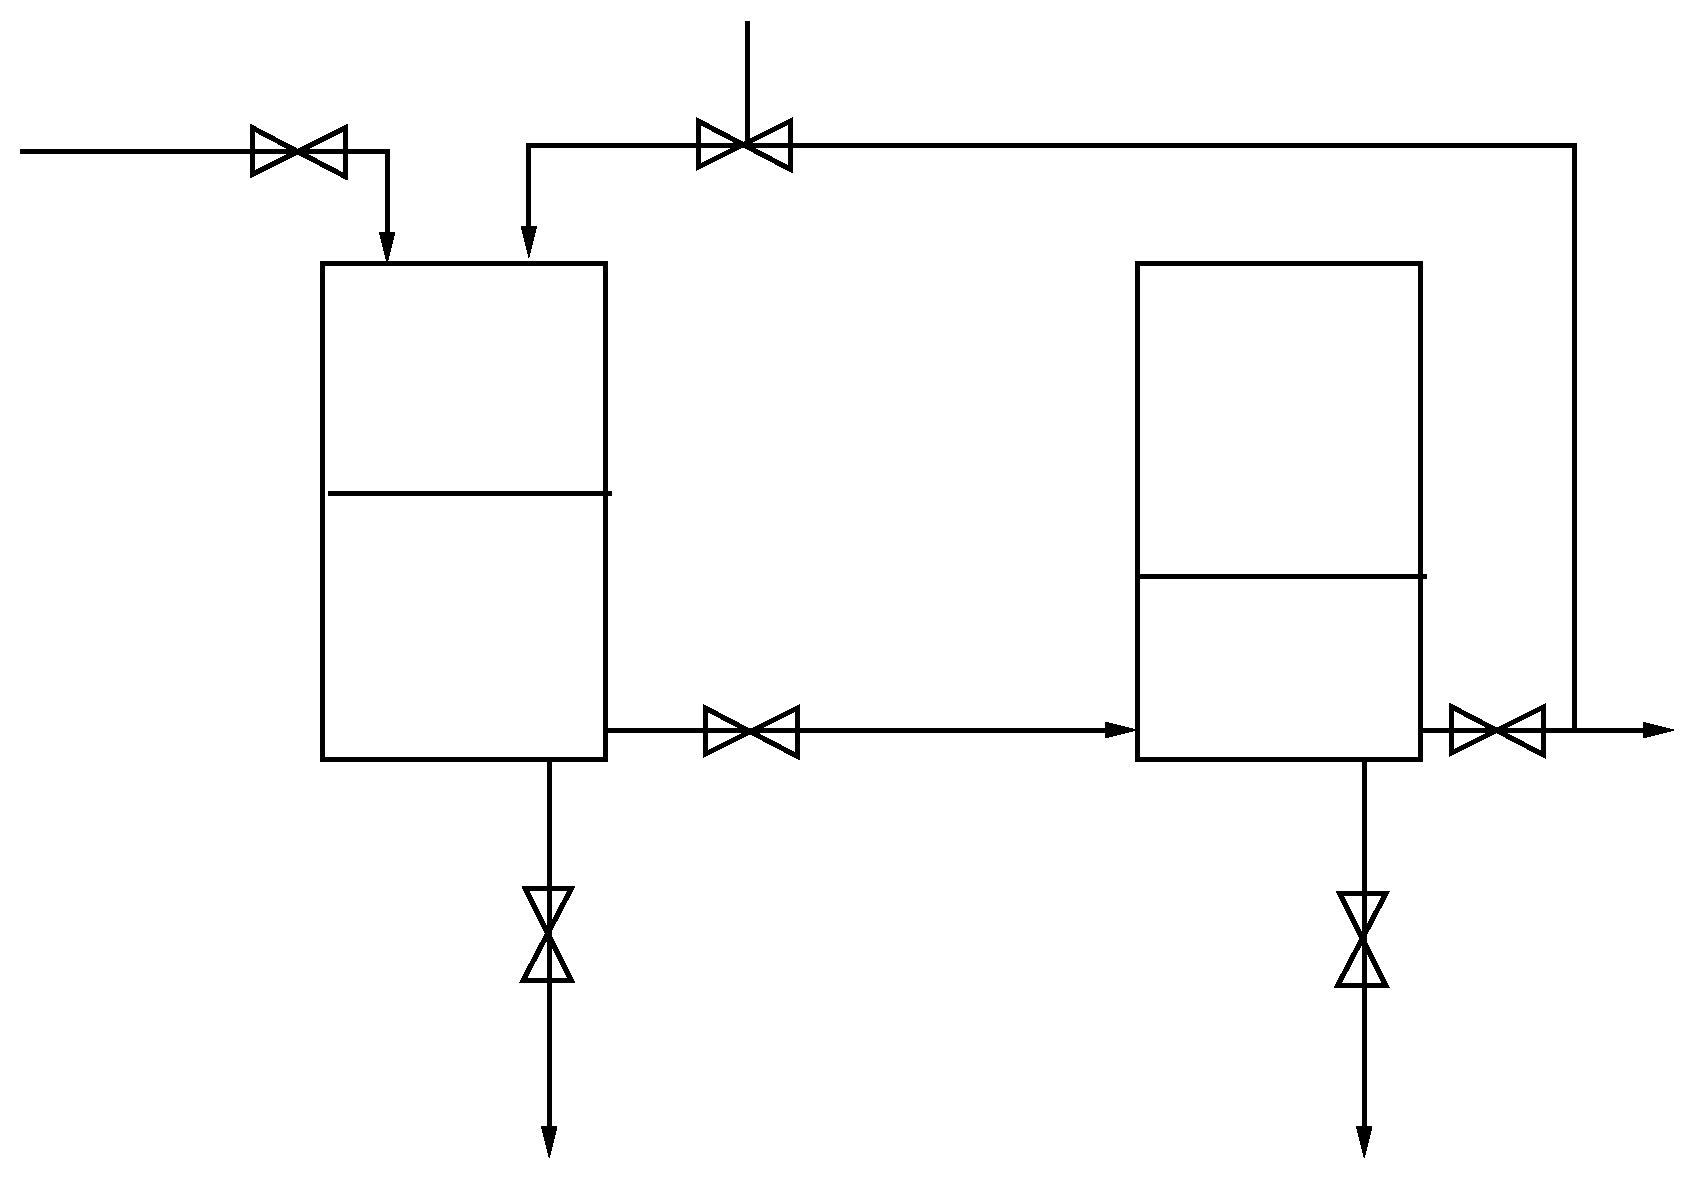
\includegraphics{mpc/2tanks_dist}%
\end{picture}%
\setlength{\unitlength}{4144sp}%
%
\begingroup\makeatletter\ifx\SetFigFont\undefined%
\gdef\SetFigFont#1#2#3#4#5{%
  \reset@font\fontsize{#1}{#2pt}%
  \fontfamily{#3}\fontseries{#4}\fontshape{#5}%
  \selectfont}%
\fi\endgroup%
\begin{picture}(12666,8726)(688,-8079)
\put(11881,-5326){\makebox(0,0)[lb]{\smash{{\SetFigFont{20}{24.0}{\rmdefault}{\mddefault}{\updefault}{\color[rgb]{0,0,0}$u_{21}$}%
}}}}
\put(1216,-646){\makebox(0,0)[lb]{\smash{{\SetFigFont{20}{24.0}{\rmdefault}{\mddefault}{\updefault}{\color[rgb]{0,0,0}$u_{11}$}%
}}}}
\put(4141,-106){\makebox(0,0)[lb]{\smash{{\SetFigFont{20}{24.0}{\rmdefault}{\mddefault}{\updefault}{\color[rgb]{0,0,0}$(1+r) u_{21}$}%
}}}}
\put(7966,-151){\makebox(0,0)[lb]{\smash{{\SetFigFont{20}{24.0}{\rmdefault}{\mddefault}{\updefault}{\color[rgb]{0,0,0}$r u_{21}$}%
}}}}
\put(9991,-4471){\makebox(0,0)[lb]{\smash{{\SetFigFont{20}{24.0}{\rmdefault}{\mddefault}{\updefault}{\color[rgb]{0,0,0}$x_2$}%
}}}}
\put(3871,-4021){\makebox(0,0)[lb]{\smash{{\SetFigFont{20}{24.0}{\rmdefault}{\mddefault}{\updefault}{\color[rgb]{0,0,0}$x_1$}%
}}}}
\put(6886,-5101){\makebox(0,0)[lb]{\smash{{\SetFigFont{20}{24.0}{\rmdefault}{\mddefault}{\updefault}{\color[rgb]{0,0,0}$u_{12}$}%
}}}}
\put(4951,-7846){\makebox(0,0)[lb]{\smash{{\SetFigFont{20}{24.0}{\rmdefault}{\mddefault}{\updefault}{\color[rgb]{0,0,0}$u_{13}$}%
}}}}
\put(11161,-7756){\makebox(0,0)[lb]{\smash{{\SetFigFont{20}{24.0}{\rmdefault}{\mddefault}{\updefault}{\color[rgb]{0,0,0}$u_{22}$}%
}}}}
\end{picture}%
}}
\caption{The two-tank system.}
\label{fig:2tankunstable}
\end{figure}

The subsystem-1 model for the two-tank system is
\begin{equation}
x_1^+ = \underbrace{1}_{A_{1}}x_1 + \underbrace{\begin{bmatrix}1 &-1 
  &-1\end{bmatrix}}_{B_{11}}\underbrace{\begin{bmatrix}u_{11}\\u_{12}\\u_{13}\end{bmatrix}}_{u_1}
+\underbrace{\begin{bmatrix}1+r &0
    \end{bmatrix}}_{B_{12}}\underbrace{\begin{bmatrix}u_{21}\\u_{22}\end{bmatrix}}_{u_2}
%\label{eq:2tanks_subsystem1}
\end{equation}
The subsystem-2 model for the two-tank system is
\begin{equation}
x_2^+ = \underbrace{1}_{A_{2}}x_2 +
\underbrace{\begin{bmatrix}0&1&0\end{bmatrix}}_{B_{21}}\underbrace{\begin{bmatrix}u_{11}\\u_{12}\\u_{13}\end{bmatrix}}_{u_1}
 +\underbrace{\begin{bmatrix}-1&-1\end{bmatrix}}_{B_{22}}\underbrace{\begin{bmatrix}u_{21}\\u_{22}\end{bmatrix}}_{u_2}
%\label{eq:2tanks_subsystem2}
\end{equation}
The overall (centralized) model of the two-tank system is the minimum
realization of
\begin{equation}
x^+ = \underbrace{\begin{bmatrix}A_1 &0\\0& A_2\end{bmatrix}}_{A}x
  + \underbrace{\begin{bmatrix}B_{11}&B_{12}\\B_{21} & B_{22} \end{bmatrix}}_{B} u
%\label{eq:centsystem}
\end{equation}
in which $x = (x_1,x_2)$ and $u =
(u_{11},u_{12},u_{13},u_{21},u_{22})$.
Each input  is constrained to lie between $[0,\bar{u}]$ in which
$0$ corresponds to the valve  completely closed and $\bar{u}$
corresponds to the valve  completely open. The upper bound on the
valve was chosen to be arbitrarily large.

We define stage costs $\ell_1(\cdot,\cdot)$ and $\ell_2(\cdot,\cdot)$:
\begin{align*}
 \ell_1(x_1,u_1)& = x_1^2+u_{11}^2+ u_{12}^2+
100u_{13}^2 \\
\ell_2(x_2,u_2)& = x_2^2+u_{21}^2+ 100u_{22}^2
\end{align*}
 
 The system starts at 
steady state with tank levels $(7,7)$ and all valves closed. At time $t=0$, we change the setpoint of the
two tanks to level $(3,3)$ and all valves closed.

The responses are shown in Figure \ref{fig:mpc:unstable}.
In noncooperative MPC, each subsystem uses the cheap input
$u_{12},u_{21}$ to change the tank levels; unaware that this choice
of inputs leads to instability by introducing more water into the
system. The subsystems manipulate the cheap inputs because the
influence of their inputs on the other subsystem is not captured in
the noncooperative MPC optimization problem.
At each iteration, the two subsystems, optimizing independently, harm each other because they do
not want to operate the expensive valves $u_{13}$ and $u_{22}$.
\begin{figure}
\centering
\scriptsize
\resizebox{\textwidth}{!}{\input{mpc/unstable_x}}
\resizebox{\textwidth}{!}{\input{mpc/unstable_u1}}
\resizebox{\textwidth}{!}{\input{mpc/unstable_u2}}
\caption{State and input profiles for two-tank system under
  distributed MPC (ncoop: noncooperative, coop: cooperative, cent: centralized).}
\label{fig:mpc:unstable}
\end{figure}
In cooperative MPC, subsystem-2 realizes that operating valve $u_{21}$
is not desirable, because it optimizes the overall objective function. The subsystems now judiciously use the expensive
valves to maintain stability.



\section{Robust cooperative MPC}
\label{sec:mpc:robust}
\subsection{Preliminaries}
We consider the centralized system \eqref{eq:mpc:distributed:cent}
obtained from the distributed models \eqref{eq:mpc:distributed:dynamics},  subject to bounded additive
disturbance as follows:
\begin{equation}
\label{eq:mpc:model_dist}
x^+ = Ax + Bu + w
\end{equation}
in which the inputs are assumed to lie in set $u_i \in \mathbb{U}_i$
as in the previous section. The assumptions on the disturbance are
stated in Assumption \ref{ass:mpc:W}

\begin{assumption}[Bounded disturbance]
\label{ass:mpc:W}
The additive disturbance $w$ lies in a convex, closed and, compact set $\mathbb{W}$
containing the origin in its interior.
\end{assumption}

The nominal system, without the additive disturbance is denoted as
follows, using $z,v$ for the nominal state and input variables.

\begin{equation}
\label{eq:mpc:model_nominal}
z^+ = Az + Bv
\end{equation}

At any time $k$, we can write the deviation between the actual state
and the nominal state as $e(k) = x(k)-z(k)$. If the inputs to both the
nominal and actual system were the same, then the error dynamics can
be written as:

\begin{equation}
\label{eq:mpc:error_dynamics}
e^+ = Ax+Bu+w - Az+Bu = Ae + w
\end{equation}

Hence, given an initial $e(0)=0$, the error at time $k$ lies in the
following set:

\begin{equation}
\label{eq:mpc:error_set}
e(k) \in S(k) :=\sum_{j=0}^{k-1}A^j\mathbb{W} = \mathbb{W} \oplus A\mathbb{W}
\oplus \ldots \oplus A^{k-1}\mathbb{W}
\end{equation}
in which $A^j\mathbb{W}$ indicates set multiplication. That is,

\[A^j\mathbb{W} := \set{A^jw \mid \forall w \in \mathbb{W}}
\]

The symbol $\oplus$ indicates set addition. That is,
\[ \mathbb{W} \oplus A\mathbb{W} := \set{w_1+w_2 \mid w_1 \in
  \mathbb{W}, w_2 \in A\mathbb{W}}\]

For stable $A$, it can be shown that the set $S(\infty)$ exists and is
positive invariant for the system \eqref{eq:mpc:error_dynamics}
\citep{kolmanovsky:gilbert:1998}.


\subsection{Tube based MPC}

We now discuss tube based MPC \citep[Chapter 3]{rawlings:mayne:2009}, the basic idea for which is as follows: (i)
use MPC on the nominal system to find $v(k) = \kappa(z(k))$,  and (ii)
based on the error at time $k$, $e(k)$, find the input to the plant as $u(k) = v(k) + Ke(k)$

By design, we select a $K$ such that $A_K:=A+BK$ is Hurwitz. Such a choice
implies that the error dynamics in the closed-loop is:
\begin{equation}
\label{eq:mpc:error_CL}
e^+ = x^+-z^+=Ax+Bv+BK(x-z)+w-Az-Bv = A_Ke+w
\end{equation}

Now, since $A_K$ is stable, we can conclude that $S_K(\infty) =
\sum_{j=0}^{\infty}A_K^j\mathbb{W}$ exists and is positive invariant
for \eqref{eq:mpc:error_CL}.

The stability and convergence theorems are therefore based on the
following observations:(i) the origin is asymptotically stable for the
nominal system $z^+= Az+B\kappa(z)$ by design, (ii) the error is designed to lie in the set
$S_K(\infty)$ by the   choice of $K$ and input $u = \kappa(z) +
K(x-z)$, and (iii) the actual state $x(k); k \rightarrow \infty$
therefore belongs to the set   $\set{0} \times S_K(\infty)$

In the presence of persistent disturbance, we ensure that the states
lie inside a bounded set that we can compute offline. The name tube
based MPC comes from the fact that at each time $k$, the state $x$
lies in a ``tube'' defined by $x(k) \in z(k)\oplus S_K(\infty)$
.  

For the inputs $u = v+K(x-z)$ to remain feasible, we need to ensure
that $v$ satisfies the tighter constraints\footnote{If state constraints are present, they need to be tightened
  as well. We do not discuss state constraints because of Assumption \ref{ass:mpc:noX}.}:
\begin{equation}
\mathbb{V} := \mathbb{U} \ominus KS_K(\infty)
\end{equation}
The tighter set follows from the fact that $e = (x-z) \in
S_K(\infty)$. 

The nominal MPC problem is defined as:
\begin{align}
\tilde{\mathbb{P}}_N(z): & \min_{\mathbf{v}}V_N(z,\mathbf{v}) \nonumber \\
& \text{s.t.~} z(j+1) = Az(j) + Bv(j)&  j = \set{0,1,\ldots,N-1}\nonumber\\
& v(j) \in \mathbb{V} \label{eq:mpc:robust:PNz},
& \qquad   j = \set{0,1,\ldots,N-1}\\
&z(0) = z \nonumber \\
& z(N) \in \mathbb{Z}_f \nonumber
\end{align}
in which $\mathbb{Z}_f$ is a terminal set that satisfies Assumption
\ref{ass:mpc:bsa} and $V_N(z,\mathbf{v})$ is the cost function defined by
\eqref{eq:mpc:VN}. Let $\kappa_s(z)$ denote the input law obtained by
implementing a suboptimal MPC algorithm on \eqref{eq:mpc:robust:PNz}. Then the
origin is asymptotically stable for the closed loop $z^+ = Az+
B\kappa_s(z)$ by Theorem \ref{thm:mpc:suboptimal}. Now, if input $u =
\kappa_s(z) + K(x-z)$ is injected to the plant, then $e \in
S_K(\infty)$. Hence, we can prove that $\mathcal{A}: = \set{0} \times
S_K(\infty)$ is asymptotically stable for the composite system 
\begin{align}
z^+ &= Az + B\kappa_s(z)\\
x^+ &= Ax + B\kappa_s(z) + BK(x-z) + w 
\end{align}

The region of attraction is $\mathcal{Z}_N \times \mathcal{X}_N$, in
which $\mathcal{Z}_N$ is the following projection:
\[ \mathcal{Z}_N : = \set{z \mid \mathbf{v} \in \mathbb{V}^N \text{s.t.~}
  z(N;z,\mathbf{v}) \in \mathbb{Z}_f}\]
and $\mathcal{X}_N := \mathcal{Z}_N \oplus S_K(\infty)$.

\subsection{Main results}
Recall that if we use the relaxation formulation to remove the
terminal region constraints in cooperative MPC, then each-time the
warm start becomes infeasible, we need a warm start recovery step,
which is the following projection onto convex sets problem:
\[ \set{\tilde{\bu}(x) \mid V_N^\beta(x,\tilde{\bu})\leq \bar{V}, \tilde{\bu}_i \in
  \mathbb{U}_i \forall i \in \set{1,2,\ldots,M}}\]
Distributed algorithms for projection onto convex sets or the convex
feasibility problems recover feasibility only at convergence. Hence,
such algorithms are not suitable for distributed warm-start
re-initialization since we cannot guarantee convergence within the
sampling time. 

To overcome these problems, we propose tube based robust cooperative
MPC that is based on two important observations:(i)  the optimization problems in tube based MPC are based on the
  nominal system, and (ii) by design, the warm start is feasible for $z^+$ if the input $v
  = \mathbf{v}(0;z)$ is implemented for the nominal system. Hence, we
  can conclude that the warm start based on the nominal MPC, $\tilde{\mathbf{v}}$, always remains feasible for the nominal problem. Furthermore, as we
discussed in Section \ref{sec:mpc:distributed:coop}, cooperative MPC stabilizes
the nominal system. Hence, we can use cooperative MPC for the nominal
system. The only caveat is that to ensure convergence to the
centralized solution, we need to have that the input sets are
uncoupled. In this case, if we wish to implement cooperative MPC on
the nominal system, we need to have that the set $\mathbb{V}$ be
uncoupled, that is 
\[ \mathbb{V} = \mathbb{V}_1 \times \mathbb{V}_2 \times \ldots \times
\mathbb{V}_M \]

In tube based MPC, the tightened set $\mathbb{V}$ is dependent
on $K$, $S_K(\infty)$ and the original disturbance set $\mathbb{W}$. So,
there is no guarantee that $\mathbb{V}$ does not have coupling between
the inputs. Therefore, we introduce another offline calculation, which
is to find a hyperbox $\tilde{\mathbb{V}}$ that lies completely inside $\mathbb{V}$. 

\begin{remark}
As shown in \citet{rakovic:kerrigan:kouramas:mayne:2003}, it is not necessary to
calculate $S_K(\infty)$ to obtain approximations to $\mathbb{V}$. In
fact, if the input constraints are polytopic and decoupled, then the
procedure mentioned in
\citet{rakovic:kerrigan:kouramas:mayne:2003}, can be used to obtain
tightened constraints that  are also polytopic and decoupled.
\end{remark} 

As noted earlier, in robust MPC, the optimizations are performed based
on the nominal state information, while the actual state could have
drifted far from the nominal state because of the disturbances. We
therefore use the modified version of the robust MPC algorithm
presented in \citet[P.234]{rawlings:mayne:2009}. 

We choose $\bar{V}, a, \beta$ such that the set 
\[\mathbb{Z}_f := \set{z \mid V_f(z) \leq a} \]
satisfies Assumption \ref{ass:mpc:bsa}. We choose $\bar{V} \geq a$ and
$\beta$ according to Proposition
\ref{prop:mpc:distributed:relaxation:betabar}. The controller gain $K$
is chosen such that the centralized system $(A+BK)$ is stable and the input constraint
set is tightened as:
\[ \tilde{\mathbb{V}} := \tilde{\mathbb{V}}_1 \times
\tilde{\mathbb{V}}_2 \times \ldots \tilde{\mathbb{V}}_M \subseteq
\mathbb{V} := \mathbb{U} \ominus KS_K(\infty) \]


The centralized nominal MPC optimization problem is: 
\begin{align}
\tilde{\mathbb{P}}_N(z): & \min_{\mathbf{v}}V^\beta_N(x,\mathbf{v}) \nonumber \\
& \text{s.t.~} z(j+1) = Az(j) + Bv(j)&   j  =  \set{0,1,\ldots,N-1}\nonumber\\
& v(j) \in \tilde{\mathbb{V}}&  j \set{\in 0,1,\ldots,N-1}  \label{eq:mpc:PNzbeta} \\
& z(0) = z \nonumber
\end{align}
Note that the region of attraction for the cooperative nominal MPC is:
\[ \mathcal{Z}_N : = \set{z \mid \mathbf{v} \in \tilde{\mathbb{V}} \text{s.t.~}
 V_N^\beta(z,\mathbf{v}) \leq \bar{V}}\]

The robust cooperative MPC algorithm is presented in Algorithm \ref{alg:mpc:robust}.
%\begin{algo}[Robust cooperative MPC] \mbox{ }
\begin{algorithm}
 \KwData{Starting state $x(0)$, initial guess
   $(\tilde{\bu}_1(0),\tilde{\bu}_2(0),\ldots,\tilde{\bu}_M(0))$ so
   that $V_N^\beta(x,\tilde{\bu}) \leq \bar{V}$
   $\bar{p} \geq 1$ and $\omega_i \in (0,1)$ such that
   $\sum_{i=0}^{M}\omega_i = 1$}
 \KwResult{Asymptotically stable closed loop}
 {\KwSty{Offline:}} Perform the following computations and share with
 every subsystem
 \Begin{
  Compute $K$ so that $A+BK$ is stable\\
  Compute/ Approximate  $S_K(\infty)$, $\mathbb{V} = \mathbb{U} \ominus KS_K(\infty)$\\
  %Compute/ Approximate $\mathbb{V} = \mathbb{U} \ominus KS_K(\infty)$\\
  Compute $\tilde{\mathbb{V}}_i$ so that $\tilde{\mathbb{V}}_1 \times
  \tilde{\mathbb{V}}_2 \times \ldots \times \tilde{\mathbb{V}}_M 
  \subseteq \mathbb{V}$\\
 }
{\KwSty{Online:}}
\Begin{
 set $z(0) \leftarrow x(0); \tilde{\mathbf{v}}(0) \leftarrow \tilde{\bu}(0)$\\
 set $k \leftarrow 0$\\
 \While {$k \geq 0$}{
   Set $p \leftarrow 0$\\
   Set $\mathbf{v}_i^{(p)} \leftarrow \tilde{\mathbf{v}}_i(k)$ for $i = 1,2,\ldots,M$\\
   Broadcast current subsystem inputs $\tilde{\mathbf{v}}_i(k)$ to other
   subsystems\\
   \While {$p < \bar{p}$}{
       \If {$V_N^\beta(x(k),\tilde{\mathbf{v}}) \leq
         V_N^\beta(z(k),\tilde{\mathbf{v}})\leq \bar{V}$}{
         \KwSty{Reset} $z(k) \leftarrow x(k)$\\
         }
         Solve $\min_{\mathbf{v}_i}V_N^\beta(z,\mathbf{v}) \text{s.t.~}
         \mathbf{v}_i \in \tilde{\mathbb{V}}_i, \mathbf{v}_{-i} =
         \mathbf{v}_{-i}^{(p)}$ to obtain $\mathbf{v}_i^0$ for i in $1,2,\ldots,M$.
         Set $\mathbf{v}_i^{(p+1)} \leftarrow \omega_i \mathbf{v}_i^{(p)} +
         (1-\omega_i) \mathbf{v}_i^0$ for i in $1,2,\ldots,M$ \\
      }
  Set $\mathbf{v} \leftarrow (\mathbf{v}_1^{(p)},\mathbf{v}_2^{(p)},\ldots,\mathbf{v}_M^{(p)})$ and find $z(k+N) \leftarrow
  \phi(N;z(k),\mathbf{v})$\\
  Obtain $v_+ = (v_{1+},v_{2+},\ldots,v_{M+}) \leftarrow \kappa_f(z(k+N))$\\
  Obtain warm start $\tilde{\mathbf{v}}_i(k+1) =
    (\mathbf{v}_i^{(p)}(1),\mathbf{v}_i^{(p)}(2),\ldots,v_{i+})$ for $i = 1,2,\ldots,M$.\\
   Set input as $v(k) =
  (\mathbf{v}_1^{(p)}(0),\mathbf{v}_2^{(p)}(0),\ldots,\mathbf{v}_M^{(p)}(0))$\\
  Evolve nominal state from $z(k)$ to $z(k+1)$ under input $v(k)$\\
  Set input $u(k) = v(k)+ K(x(k) - z(k))$\\
  Evolve state from $x(k)$ to $x(k+1)$ under input $u(k)$\\
 }
}
\caption{Robust cooperative MPC}
\label{alg:mpc:robust}
\end{algorithm}

The modification that we alluded to earlier is the ``if condition'' in
Algorithm \ref{alg:mpc:robust}. The condition states that if the warm start
is feasible for the actual state at time $k$ and satisfies a cost-drop
criteria, then we reset the error to zero. In this way, not only do we not
lose the convergence property of the closed-loop nominal state (since
the cost-drop is satisfied all the time), but we also incorporate
feedback into the system. Another modification to Algorithm
\ref{alg:mpc:robust} is a slow time scale reset of the nominal state to the
actual state. That is, after every $T$ sampling times, in which $T$ is
much larger than the sampling time employed, we automatically reset
the nominal trajectory. However, in this case, we need to ensure that
the warm-start is feasible for the reset. 

\subsection{Example}
Consider the two tank system as shown in Figure
\ref{fig:mpc:two_tanks}. The overall system consists of two tanks which
are the two subsystems. The first subsystem (tank-1) manipulates inputs
$u_1 = (u_{11},u_{12})$, while the second subsystem (tank-2) manipulates
inputs $u_2 = (u_{22})$. There are two disturbances affecting the
system, $w_1$ in the first tank and $w_2$ in the second tank. The
state dynamics for this two tank system is given by:
\begin{equation*}
\begin{bmatrix}x_1\\x_2\end{bmatrix}^+ = \begin{bmatrix}1&\\ &
  1\end{bmatrix} \begin{bmatrix}x_1\\x_2\end{bmatrix}+
\begin{bmatrix} 1 & - 1 \\ 0&
  1 \end{bmatrix}u_1+ \begin{bmatrix}0\\-1\end{bmatrix}u_2
+ \begin{bmatrix}w_1\\w_2\end{bmatrix}
\end{equation*}

\begin{figure*}
\centering
\scriptsize
\resizebox{0.75\textwidth}{!}{\begin{picture}(0,0)%
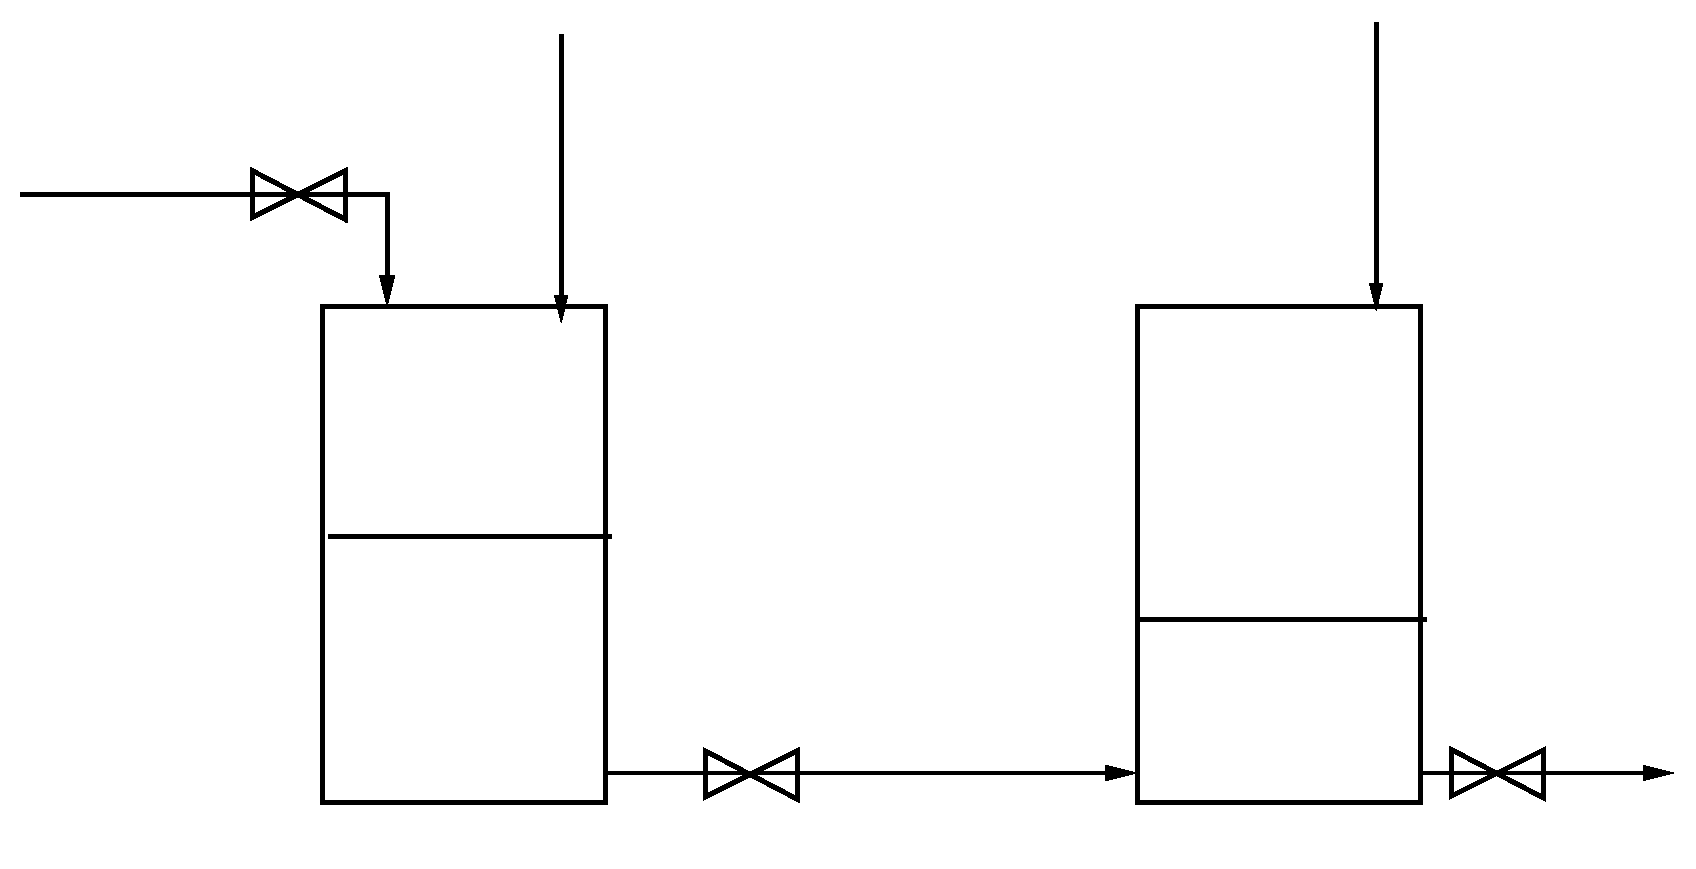
\includegraphics{two_tanks}%
\end{picture}%
\setlength{\unitlength}{4144sp}%
%
\begingroup\makeatletter\ifx\SetFigFont\undefined%
\gdef\SetFigFont#1#2#3#4#5{%
  \reset@font\fontsize{#1}{#2pt}%
  \fontfamily{#3}\fontseries{#4}\fontshape{#5}%
  \selectfont}%
\fi\endgroup%
\begin{picture}(12666,6356)(688,-5390)
\put(11881,-5326){\makebox(0,0)[lb]{\smash{{\SetFigFont{20}{24.0}{\rmdefault}{\mddefault}{\updefault}{\color[rgb]{0,0,0}$u_{22}$}%
}}}}
\put(1216,-646){\makebox(0,0)[lb]{\smash{{\SetFigFont{20}{24.0}{\rmdefault}{\mddefault}{\updefault}{\color[rgb]{0,0,0}$u_{11}$}%
}}}}
\put(9991,-4471){\makebox(0,0)[lb]{\smash{{\SetFigFont{20}{24.0}{\rmdefault}{\mddefault}{\updefault}{\color[rgb]{0,0,0}$x_2$}%
}}}}
\put(3871,-4021){\makebox(0,0)[lb]{\smash{{\SetFigFont{20}{24.0}{\rmdefault}{\mddefault}{\updefault}{\color[rgb]{0,0,0}$x_1$}%
}}}}
\put(6886,-5101){\makebox(0,0)[lb]{\smash{{\SetFigFont{20}{24.0}{\rmdefault}{\mddefault}{\updefault}{\color[rgb]{0,0,0}$u_{12}$}%
}}}}
\put(5041,-1006){\makebox(0,0)[lb]{\smash{{\SetFigFont{20}{24.0}{\rmdefault}{\mddefault}{\updefault}{\color[rgb]{0,0,0}$w_1$}%
}}}}
\put(11251,-1096){\makebox(0,0)[lb]{\smash{{\SetFigFont{20}{24.0}{\rmdefault}{\mddefault}{\updefault}{\color[rgb]{0,0,0}$w_2$}%
}}}}
\end{picture}%
}
\caption{Two tank system}
\label{fig:mpc:two_tanks}
\end{figure*}

We assume that the nominal value of $w_{1,n} = 0.1$ and that of $w_{2,n} =
5$. The set $\mathbb{W}$ is given by $\mathbb{W} := \set{w \mid 0\leq
  w_1\leq 0.2, 0 \leq w_2 \leq 10}$.

The input constraints are given by $\mathbb{U}_1 = \set {u_1 \mid 0
  \leq u_{11} \leq 10, 0 \leq u_{12} \leq 10}$ and $\mathbb{U}_2 =
\set{u_2 \mid 0 \leq u_{22} \leq 20}$.

Note that since we have a system of integrators, any level in the tank
can be stabilized as long as all the flows in the system are
balanced. Therefore, we choose the steady state in the tank as $x_s =
(20,20)$ (the level in both tanks are 20). The input steady state is
obtained by solving the following optimization problem
\[ \min_{u}{1/2u'Ru} \qquad \text{s.t.~} Bu = -w_n ; u \in \mathbb{U} \]
in which $w_n$ is the nominal disturbance. For the choice of $R = I$
($I$ denotes the identity matrix), the input steady state  is obtained
as $u_s = (3.2667,3.3667,8.3667)$. 

The stage cost was chosen as $\ell(x,u) = 1/2(0.1 x'x + u'u)$. We solve the
MPC problem in deviation variables, so that regulation to the origin
implies regulation to the steady state mentioned above. Following
the design procedure outlined in the previous sections, we choose 
(i) $V_f(x) = 1/2x'Px,\kappa_f(x) = Kx$ as the solution to the Riccati
equation, 
(ii)$a$ = 1 and the terminal region as $\set{x \mid 1/2x'Px \leq 1}$. The choice of
  $a=1$ satisfies the requirements in Assumption \ref{ass:mpc:bsa}, (iii)
$\bar{V} = 100$, (iv) a prediction horizon of $N=15$ and (v)the controller that corrects for the error between the nominal
  and actual states was as $K = \kappa_f(x)$.

For these choice of parameters, we followed the algorithm mentioned in
\citet{rakovic:kerrigan:kouramas:mayne:2003} to find the set
$\mathbb{V}$ (we chose $N=200$ and $\alpha = 1e-6$). Note that, since the original input set contained no
coupled inputs, the tightened set also contains no coupled inputs. 

In Figure \ref{fig:mpc:CL1}, we show the closed-loop response 
nominal closed-loop response of the level in the second tank and for cooperative MPC rejecting a
persistent disturbance $w_k \in \mathbb{W}$.  We also show the cost-function $V^\beta_N(z,\tilde{\mathbf{v}})$ and
$V_N^\beta(x,\tilde{\mathbf{v}})$ to show that although the warm-start was
infeasible for the actual state, it was still feasible for the nominal
state and hence we could obtain the closed-loop guarantees for robust
cooperative MPC. Note that, for this particular disturbance
realization, we could not reset the nominal state to the actual state.

\begin{figure}
\centering
\scriptsize
\resizebox{1\textwidth}{!}{\input{mpc/CL1}}
\caption{(Left) Closed-loop response (Right) Warm start rendered
  infeasible for actual state because of disturbance. The warm start
  is infeasible if $V_N^\beta(x,\tilde{\mathbf{v}})> \bar{V}$}
\label{fig:mpc:CL1}
\end{figure}


In Figure \ref{fig:mpc:CL2}, we show the closed-loop response using a
modified version of Algorithm \ref{alg:mpc:robust}. The modification we
made are to reset the nominal state to the actual state at time $k$ if the
following conditions are satisfied (i)The nominal state $z(k)$ is inside $\mathbb{Z}_f$.
(ii) The warm start $\tilde{\mathbf{v}}(k)$ is feasible for the
actual state $x(k)$ and , (iii) The time elapsed since the last reset
is greater than $\bar{T}$
time periods (we chose $\bar{T} = 10$)

\begin{figure}
\centering
\scriptsize
\resizebox{1\textwidth}{!}{% GNUPLOT: LaTeX picture with Postscript
\begingroup
  \makeatletter
  \providecommand\color[2][]{%
    \GenericError{(gnuplot) \space\space\space\@spaces}{%
      Package color not loaded in conjunction with
      terminal option `colourtext'%
    }{See the gnuplot documentation for explanation.%
    }{Either use 'blacktext' in gnuplot or load the package
      color.sty in LaTeX.}%
    \renewcommand\color[2][]{}%
  }%
  \providecommand\includegraphics[2][]{%
    \GenericError{(gnuplot) \space\space\space\@spaces}{%
      Package graphicx or graphics not loaded%
    }{See the gnuplot documentation for explanation.%
    }{The gnuplot epslatex terminal needs graphicx.sty or graphics.sty.}%
    \renewcommand\includegraphics[2][]{}%
  }%
  \providecommand\rotatebox[2]{#2}%
  \@ifundefined{ifGPcolor}{%
    \newif\ifGPcolor
    \GPcolortrue
  }{}%
  \@ifundefined{ifGPblacktext}{%
    \newif\ifGPblacktext
    \GPblacktexttrue
  }{}%
  % define a \g@addto@macro without @ in the name:
  \let\gplgaddtomacro\g@addto@macro
  % define empty templates for all commands taking text:
  \gdef\gplbacktext{}%
  \gdef\gplfronttext{}%
  \makeatother
  \ifGPblacktext
    % no textcolor at all
    \def\colorrgb#1{}%
    \def\colorgray#1{}%
  \else
    % gray or color?
    \ifGPcolor
      \def\colorrgb#1{\color[rgb]{#1}}%
      \def\colorgray#1{\color[gray]{#1}}%
      \expandafter\def\csname LTw\endcsname{\color{white}}%
      \expandafter\def\csname LTb\endcsname{\color{black}}%
      \expandafter\def\csname LTa\endcsname{\color{black}}%
      \expandafter\def\csname LT0\endcsname{\color[rgb]{1,0,0}}%
      \expandafter\def\csname LT1\endcsname{\color[rgb]{0,1,0}}%
      \expandafter\def\csname LT2\endcsname{\color[rgb]{0,0,1}}%
      \expandafter\def\csname LT3\endcsname{\color[rgb]{1,0,1}}%
      \expandafter\def\csname LT4\endcsname{\color[rgb]{0,1,1}}%
      \expandafter\def\csname LT5\endcsname{\color[rgb]{1,1,0}}%
      \expandafter\def\csname LT6\endcsname{\color[rgb]{0,0,0}}%
      \expandafter\def\csname LT7\endcsname{\color[rgb]{1,0.3,0}}%
      \expandafter\def\csname LT8\endcsname{\color[rgb]{0.5,0.5,0.5}}%
    \else
      % gray
      \def\colorrgb#1{\color{black}}%
      \def\colorgray#1{\color[gray]{#1}}%
      \expandafter\def\csname LTw\endcsname{\color{white}}%
      \expandafter\def\csname LTb\endcsname{\color{black}}%
      \expandafter\def\csname LTa\endcsname{\color{black}}%
      \expandafter\def\csname LT0\endcsname{\color{black}}%
      \expandafter\def\csname LT1\endcsname{\color{black}}%
      \expandafter\def\csname LT2\endcsname{\color{black}}%
      \expandafter\def\csname LT3\endcsname{\color{black}}%
      \expandafter\def\csname LT4\endcsname{\color{black}}%
      \expandafter\def\csname LT5\endcsname{\color{black}}%
      \expandafter\def\csname LT6\endcsname{\color{black}}%
      \expandafter\def\csname LT7\endcsname{\color{black}}%
      \expandafter\def\csname LT8\endcsname{\color{black}}%
    \fi
  \fi
  \setlength{\unitlength}{0.0500bp}%
  \begin{picture}(7200.00,3024.00)%
    \gplgaddtomacro\gplbacktext{%
      \csname LTb\endcsname%
      \put(814,704){\makebox(0,0)[r]{\strut{} 10}}%
      \put(814,1732){\makebox(0,0)[r]{\strut{} 20}}%
      \put(814,2759){\makebox(0,0)[r]{\strut{} 30}}%
      \put(946,484){\makebox(0,0){\strut{} 0}}%
      \put(1433,484){\makebox(0,0){\strut{} 10}}%
      \put(1921,484){\makebox(0,0){\strut{} 20}}%
      \put(2408,484){\makebox(0,0){\strut{} 30}}%
      \put(2896,484){\makebox(0,0){\strut{} 40}}%
      \put(3383,484){\makebox(0,0){\strut{} 50}}%
      \put(176,1731){\rotatebox{-270}{\makebox(0,0){\strut{}Level in Tank-1}}}%
      \put(2164,154){\makebox(0,0){\strut{}Time}}%
      \put(1921,1218){\makebox(0,0)[l]{\strut{}$S_K(\infty)$ bound}}%
    }%
    \gplgaddtomacro\gplfronttext{%
      \csname LTb\endcsname%
      \put(2396,2586){\makebox(0,0)[r]{\strut{}Actual}}%
      \csname LTb\endcsname%
      \put(2396,2366){\makebox(0,0)[r]{\strut{}Nominal}}%
    }%
    \gplgaddtomacro\gplbacktext{%
      \csname LTb\endcsname%
      \put(4109,484){\makebox(0,0){\strut{} 0}}%
      \put(4517,484){\makebox(0,0){\strut{} 2}}%
      \put(4925,484){\makebox(0,0){\strut{} 4}}%
      \put(5334,484){\makebox(0,0){\strut{} 6}}%
      \put(5742,484){\makebox(0,0){\strut{} 8}}%
      \put(6150,484){\makebox(0,0){\strut{} 10}}%
      \put(6282,704){\makebox(0,0)[l]{\strut{} 0}}%
      \put(6282,1115){\makebox(0,0)[l]{\strut{} 100}}%
      \put(6282,1526){\makebox(0,0)[l]{\strut{} 200}}%
      \put(6282,1937){\makebox(0,0)[l]{\strut{} 300}}%
      \put(6282,2348){\makebox(0,0)[l]{\strut{} 400}}%
      \put(6282,2759){\makebox(0,0)[l]{\strut{} 500}}%
      \put(7051,1731){\rotatebox{-270}{\makebox(0,0){\strut{}Cost}}}%
      \put(5129,154){\makebox(0,0){\strut{}Time}}%
    }%
    \gplgaddtomacro\gplfronttext{%
      \csname LTb\endcsname%
      \put(5163,2586){\makebox(0,0)[r]{\strut{}$V_N^\beta(x,\tilde{\mathbf{v}})$}}%
      \csname LTb\endcsname%
      \put(5163,2366){\makebox(0,0)[r]{\strut{}$V_N^\beta(z,\tilde{\mathbf{v}})$}}%
      \csname LTb\endcsname%
      \put(5163,2146){\makebox(0,0)[r]{\strut{}$\bar{V}$}}%
    }%
    \gplbacktext
    \put(0,0){\includegraphics{mpc/CL2}}%
    \gplfronttext
  \end{picture}%
\endgroup
}
\caption{(Left) Closed-loop response. Notice that we reset the state
  around t = 15 (Right) Warm start rendered
  infeasible for actual state because of disturbance}
\label{fig:mpc:CL2}
\end{figure}





\section{Related Work}
\label{sec:mpc:related}
Cooperative MPC has evolved as an  attractive architecture for
distributed control because it solves the centralized control
problem, and inherits the desirable closed-loop properties of
centralized control. 
In the previous sections, we described
cooperative MPC based on the ``primal decomposition'' of the
centralized optimization
problem. In the primal decomposition, the centralized optimization
problem is solved directly using parallel optimization
architectures. \citet{liu:chen:pena:christofides:2010} also use the
primal decomposition to solve the centralized optimization problem for a
nonlinear process model. They use a closed-form controller $u=h(x)$
for which a Lyapunov function is known as a reference controller to
design their MPC optimization problem. Thus, they ensure that the MPC
inherits the stability properties of $u=h(x)$. Note that $u=h(x)$ also
provides a warm start, even when the actual and predicted states are
different. However, since this stability constraint is a coupled
constraint, there can be no guarantees about the convergence of the
parallel optimization routine to the optimal solution; and hence equivalence of optimal MPC
and cooperative MPC if the iterations were allowed to converge. The authors propose both a Jacobi
algorithm (all subsystems optimize in parallel) and a Gauss-Seidel
algorithm (subsystems optimize in sequence). In comparison, in
\citet{stewart:wright:rawlings:2011}, the authors propose a Jacobi
algorithm for nonlinear MPC that converges to the centralized optimal
solution. Since, for non-convex problems, the Jacobi optimizations
does not necessarily produce a descent direction, the authors propose
a sequential procedure to obtain a descent direction using the
solutions obtained from each subsystem. This overhead is not
equivalent to implementing a coordinator as each subsystem only
calculates an objective function in the second phase of the algorithm
in which a descent direction is
determined. \citet{maestre:pena:camacho:alamo:2011} propose a primal
decomposition approach to cooperative MPC based on agent
negotiation. The advantage of their procedure is that agents need only
know models of the subsystems whose inputs affect their states. In the
proposed method, each agent optimizes its local objective over all
the inputs that affect its dynamics, and share the proposed solution
with other agents. The other agents evaluate the proposal for
cost-drop and constraint violation and communicate back to the
original agent making the proposal, who can then decide to accept or
reject the proposal. The authors ensure that only feasible proposals
are accepted. The drawback of the proposed architecture, however, is
that (i) the agents have to solve larger optimization problems
(because they have to optimize over all the inputs that affect their
state), and (ii) the convergence to the centralized optimal solution
cannot be guaranteed. Stability is guaranteed using the warm
start. \citet{maestre:pena:camacho:2011} use game-theoretic analysis
to propose a distributed optimization framework. In this method, each
node, optimizes its local objective over its local decisions while
keeping the other subsystem decisions fixed. After completion of the
optimizations, the agents compute their local objectives for all
possible combinations of the overall system input (based on optimized
solution of the agents and the warm start). Upon sharing the
objectives, the agents then select the input that minimizes the
overall cost. Thus, each agent cooperatively makes a decision. However,
the proposed algorithm also fails to establish convergence to the
centralized optimal on iteration. Stability is guaranteed by design of
terminal region and warm-start. \citet{muller:revle:allgower:2012}
propose a optimization algorithm based on each node optimizing over
its local optimization problem. They use a terminal region which is a
sub-level set of the terminal penalty. Because of the presence of
coupled constraints, input directions are discarded if they are not
feasible, based on a check made after the optimizations. To ensure
cost-drop, the centralized objectives are also evaluated after the
optimizations and inputs that do not achieve cost-drop are
discarded. The model considered by the authors had coupling introduced
only via the constraints (both in the objective function and the
constraints). The authors also provide a method to define local time
varying terminal regions, so that the coupled terminal region
constraint is satisfied if each subsystem satisfies its local time
varying terminal region constraint. The algorithm provided by the
authors, satisfies the requirements of the optimizer for suboptimal
MPC, but again, does not give any  guarantee on convergence to the
optimal solution. The
requirement of decoupled dynamics is important in problems like multi
vehicle synchronization
etc. \citet{johansson:speranzon:johansson:johansson:2006} use a primal
decomposition to solve a multi-vehicle consensus problem as a MPC
problem. While the dynamics are decoupled, the consensus point,
similar to terminal equality constraint, is the complicating
constraint. Unlike the MPC problems where the objectives are also
constrained because of the dynamics, the multi-vehicle receding
horizon problem falls into the category of uncoupled objective but
coupled constraints. The author's use a primal decomposition which
generates feasible iterate that reduce the objective function
value. However, in order to ensure that the centralized optimal
solution is achieved, the authors use a coordinator, which is based on
sub-gradient optimization to handle the coupled constraint.

A common theme in optimizing the centralized  problem is
that it is not easy to guarantee convergence to the optimal
solution. However, stability can be guaranteed because every iterate
is designed so that it reduces the cost while remaining feasible. In
contrast, there are a lot of cooperative MPC algorithms which are
based on the ``dual decomposition''. In the dual decomposition, the
coupled constraints are relaxed by using the Lagrangian of the
optimization problem. For a fixed value of the Lagrange multipliers
(also called as prices or dual variables), the relaxed problem can be solved using
parallel optimization methods as there are no complicating
constraints. Upon achieving the solution to the relaxed problem, the
Lagrange multipliers are updated. The Lagrange multiplier update is
usually done by a coordinator. These algorithms often converge faster
to the optimal solution. However, their main disadvantage is that they
are guaranteed to produce a feasible iterate only upon
convergence. Since stability theory for suboptimal MPC rely on the
fact that the suboptimal iterate is feasible, cooperative MPC
algorithms using dual decomposition use stability theory based on
optimal MPC to ensure stability. Therefore, a common theme in dual
decomposition based cooperative MPC algorithms are a coordinator layer
and a requirement that the iterates converge. 

The cooperative MPC algorithms using dual decomposition differ based on
the technique used to update the dual variables. In
\citet{cheng:forbes:yip:2007}, the dual variables (prices) are updated
using a sub-gradient based optimization algorithm. Sub-gradient methods
are also used in \citet{ma:anderson:borrelli:2011},
\citet{wakasa:arakawa:tanka:akashi:2008},
\citet{marcos:forbes:guay:2009}. \citet{morocan:bourdais:dumur:buisson:2011}
formulate the building control problem as a MPC problem with linear
objectives and use Benders decomposition to solve the problem. Benders
decomposition is a widely popular parallel algorithm when by fixing the
value of a complicating variable, the remaining problem can be
completely separated. \citet{scheu:marquardt:2011} propose a dual
decomposition algorithm without a coordination layer. They augment the
local subsystem objective function with the sensitivity of the
objectives and constraints of other subsystems to obtain updates for
the dual variables along with the primal variables. However, this
method generates a feasible solution only upon
convergence. \citet{giselsson:doan:keviczky:schutter:rantzer:2012}, \citet{giselsson:rantzer:2010}
propose a dual decomposition algorithm with a stopping criteria based
on the objective value to ensure stability. They advocate the use of
long prediction horizon along with results obtained in
\citet{grune:2009} to determine bounds on the value of the objective
function so that stability can be
guaranteed. \citet{doan:keviczky:necoara:diehl:schutter:2009} modified
the Han's algorithm which is a dual decomposition based algorithm for
the special structure of the MPC problem. Although the method uses
communication between directly connected subsystems, stability is
guaranteed only upon convergence. \citet{necoara:doan:suykens:2008}
use a smoothing technique to simplify the dual problem. With the
smoothing technique, the coordinator problem for finding the Lagrange
multiplier updates becomes easier. The algorithm also gives bounds on
the number of iterations so that the optimal solution and constraint
violation are within a pre-specified limit ($\epsilon$ approximation of
the centralized problem). Finally, \citet{doan:keviczky:schutter:2011}, propose a primal feasible dual
gradient approach, that generates a primal feasible solution  that
achieves cost-drop in a
finite number of iterations based on an averaging scheme of the primal
variables at each iteration. 

\citet{christofides:scattolini:pena:liu:2012} is a recent review of different algorithms for distributed
MPC. \citet{necoara:nedelcu:dumitrache:2011} provides an excellent overview of the different
optimization problems and parallel solution strategies that are seen
in control and estimation.

\citet{trodden:richards:2006,trodden:richards:2007} propose a tube based robust distributed
MPC algorithm. In their method, at each sampling time, only one
subsystem performs optimization. The subsystem optimizes only over its
decision variables, keeping all other subsystem decisions fixed from
the previous iteration. This method is also an example of primal
decomposition. \citet{richards:how:2004} present a robust tube-based
MPC for systems with decoupled dynamics. The coupling constraints are
coupled output constraints. Their algorithm is based on the
Gauss-Seidel iterations.

